\section{Implementation Results}

\label{sec:results}

\subsection{Evidence and Selected Experiments}

\begin{itemize}
\setlength{\itemsep}{3pt}
\setlength{\parskip}{0pt}
\item \textbf{Evidence.} The main comparison uses the exact five runs identified in the \texttt{a1} README and committed comparison CSV at revision \texttt{27ef182}~\cite{code}.
\item \textbf{Selected runs.} Linear uses \texttt{linear\_baseline\_001}; MLP, CNN, LSTM and Transformer use their respective \texttt{baseline\_002} runs.
\item \textbf{Checkpoint protocol.} All have 20 logged epochs and a validation-selected checkpoint. Run identifiers distinguish saved experiments; a suffix is not a random-seed number.
\end{itemize}


\subsection{Training Behavior}

\subsubsection{Learning Curves and Selected Checkpoints}

\begin{itemize}
\setlength{\itemsep}{3pt}
\setlength{\parskip}{0pt}
\item \textbf{Learning curves.} Figures~\ref{fig:learning}--\ref{fig:learning-transformer} reproduce the learning-curve images committed in the cited branch, without redrawing them. Loss decreases and validation Macro-F1 improves substantially for every model.
\item \textbf{Checkpoint statistics.} Table~\ref{tab:bestepochs} gives values at the selected checkpoint, rather than combining training statistics from a different epoch.
\end{itemize}
\begin{table}[!htbp]\centering\small

\caption{Validation-selected checkpoints. Training accuracy is collected in training mode during the epoch; validation accuracy uses the resulting model in evaluation mode.}

\label{tab:bestepochs}

\begin{tabular}{@{}lrrrrr@{}}\toprule

Model & Epoch & Val. F1 & Train Acc. (\%) & Val. Acc. (\%) & Val. loss\\\midrule

Linear & 13 & 0.8563 & 86.38 & 85.64 & 0.4260 \\

MLP & 20 & 0.8970 & 92.61 & 89.63 & 0.3082 \\

CNN & 19 & 0.9226 & 94.53 & 92.22 & 0.2343 \\

LSTM & 20 & 0.8990 & 92.25 & 89.90 & 0.2971 \\

Transformer & 17 & 0.8910 & 91.01 & 89.11 & 0.3140 \\

\bottomrule\end{tabular}\end{table}



\begin{itemize}
\setlength{\itemsep}{3pt}
\setlength{\parskip}{0pt}
\item \textbf{Selected epochs.} Linear peaks at epoch 13 and Transformer at epoch 17; their last epochs are not automatically the selected models. CNN's best validation Macro-F1 is at epoch 19, while MLP and LSTM select epoch 20.
\item \textbf{Training budget and interpretation.} None uses early stopping: all complete their full budget. Selecting epoch 20 for MLP/LSTM leaves open whether a longer budget would help; it does not establish non-convergence.
\end{itemize}


\par\medskip\noindent\begin{minipage}{\linewidth}

\centering

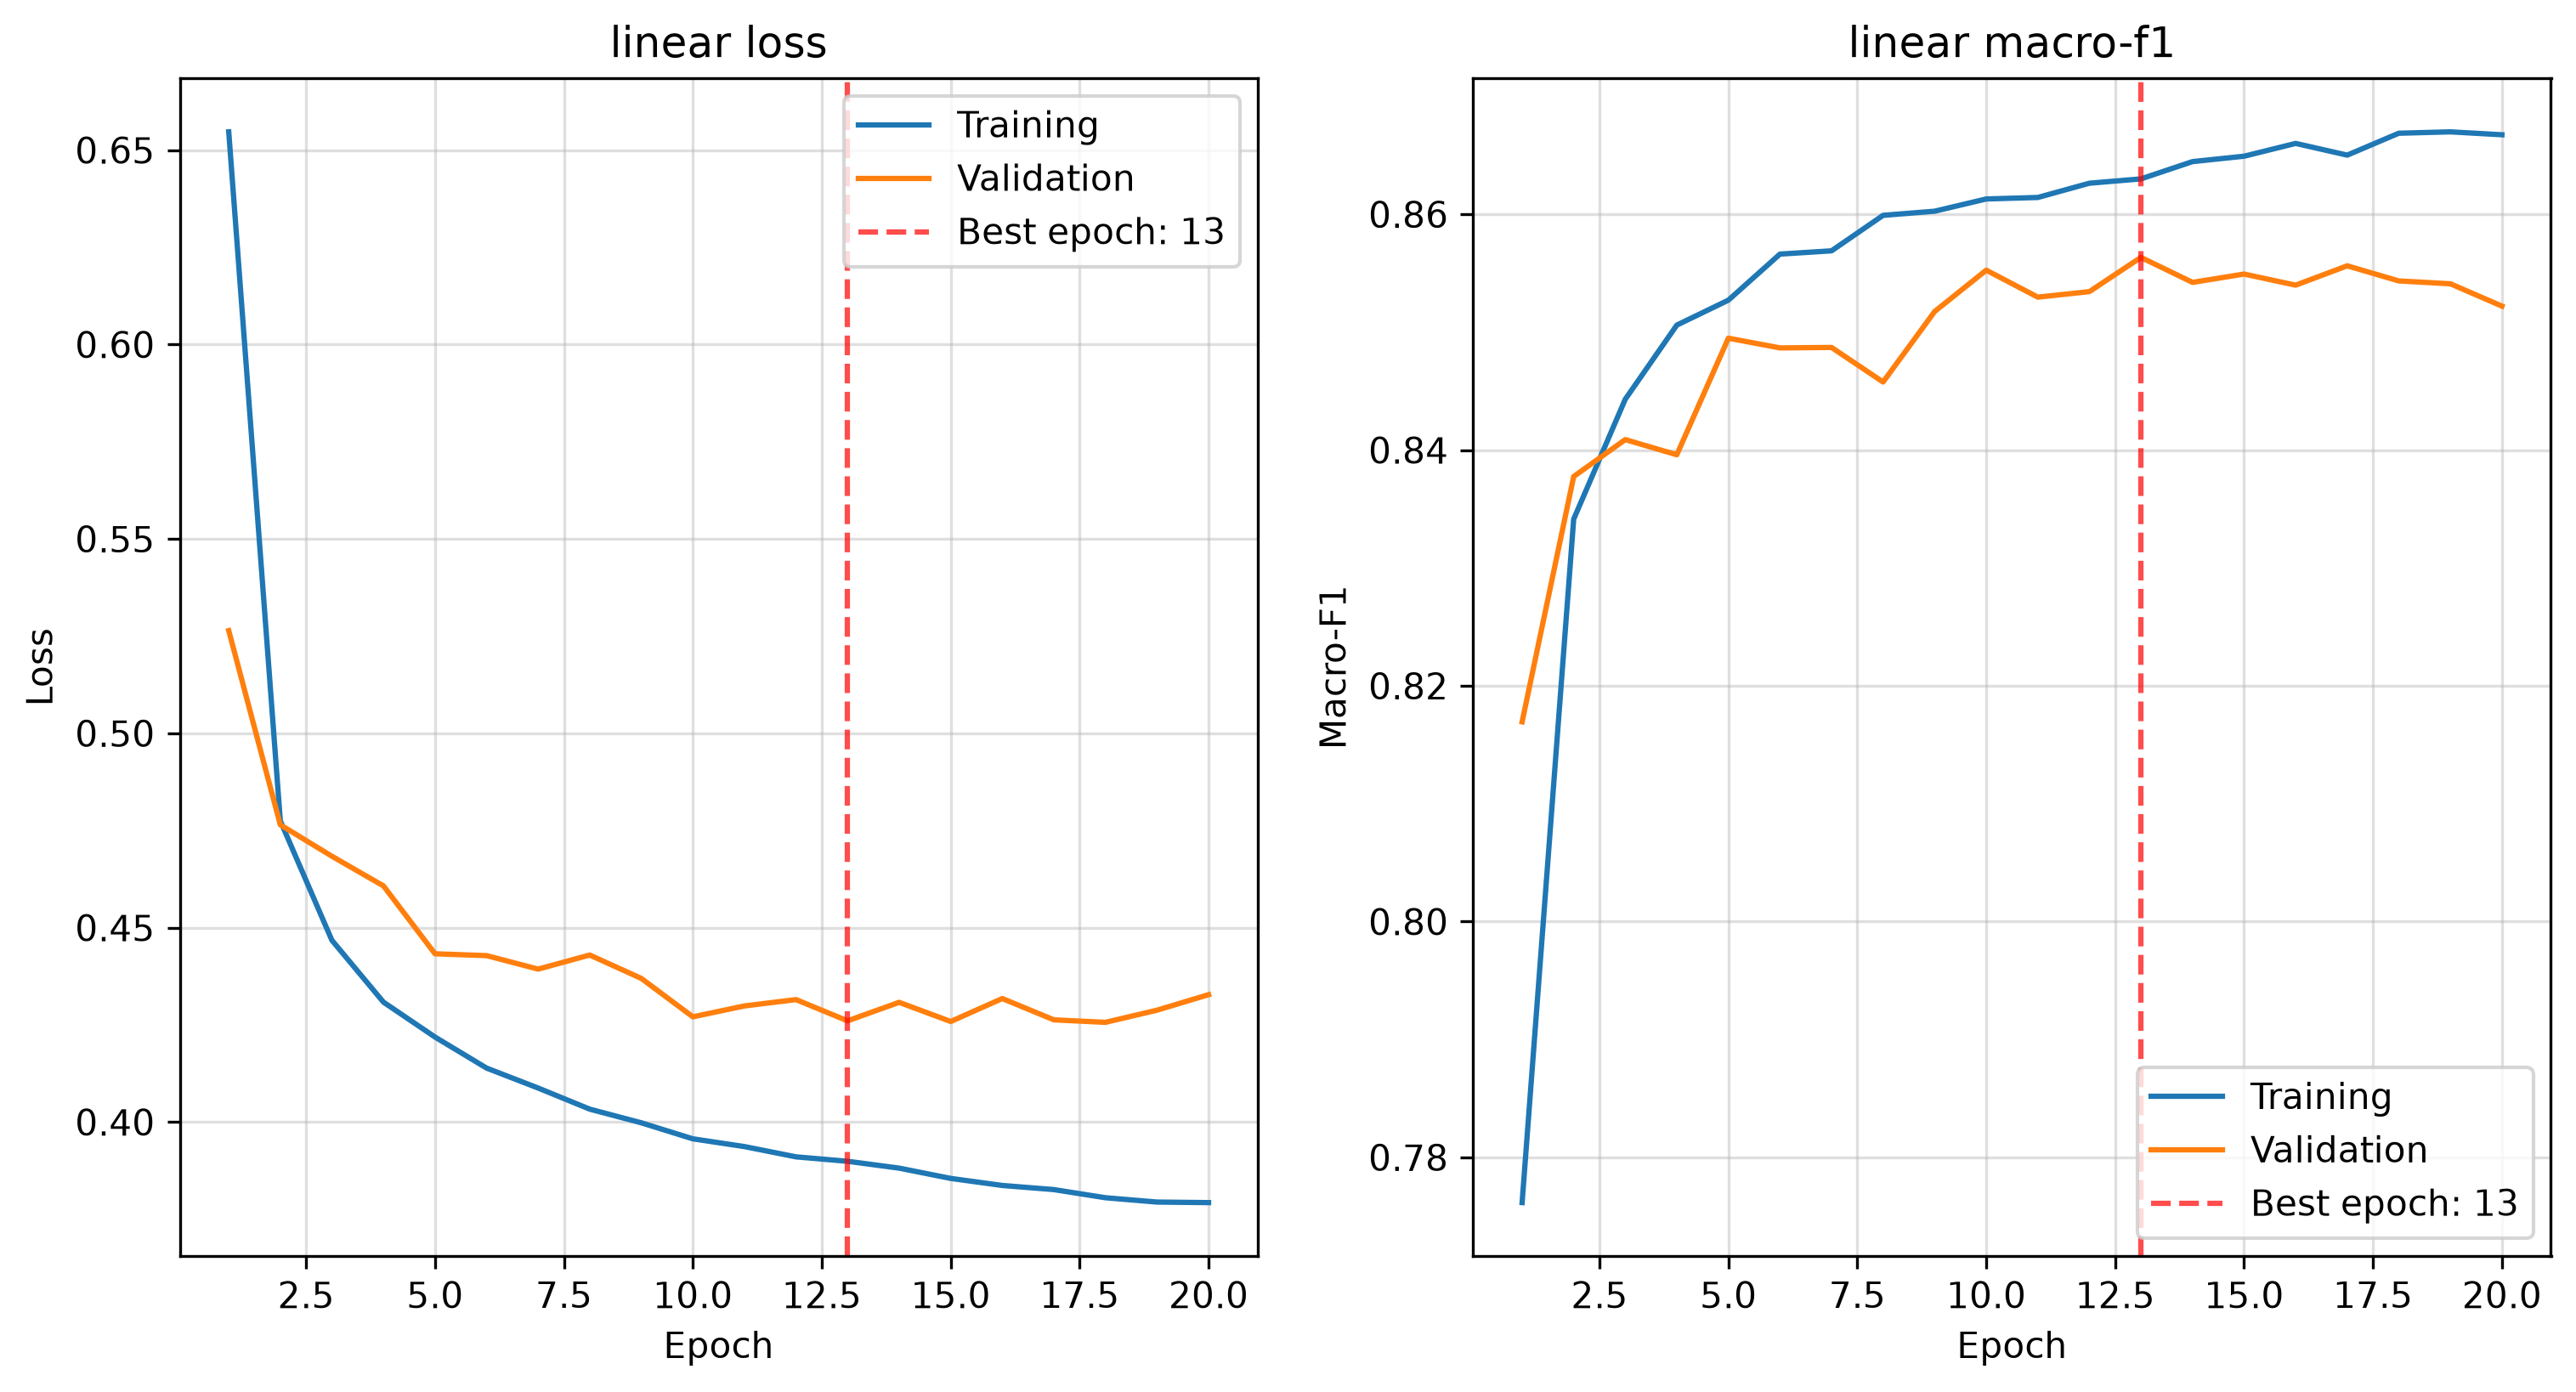
\includegraphics[width=\linewidth]{images/final_linear_baseline_001_learning_curves.png}

\captionof{figure}{Linear: original training/validation loss and Macro-F1 curves from branch \texttt{a1}. The red dashed line marks the validation-selected epoch.}

\label{fig:learning}

\end{minipage}\par\medskip



\par\medskip\noindent\begin{minipage}{\linewidth}

\centering

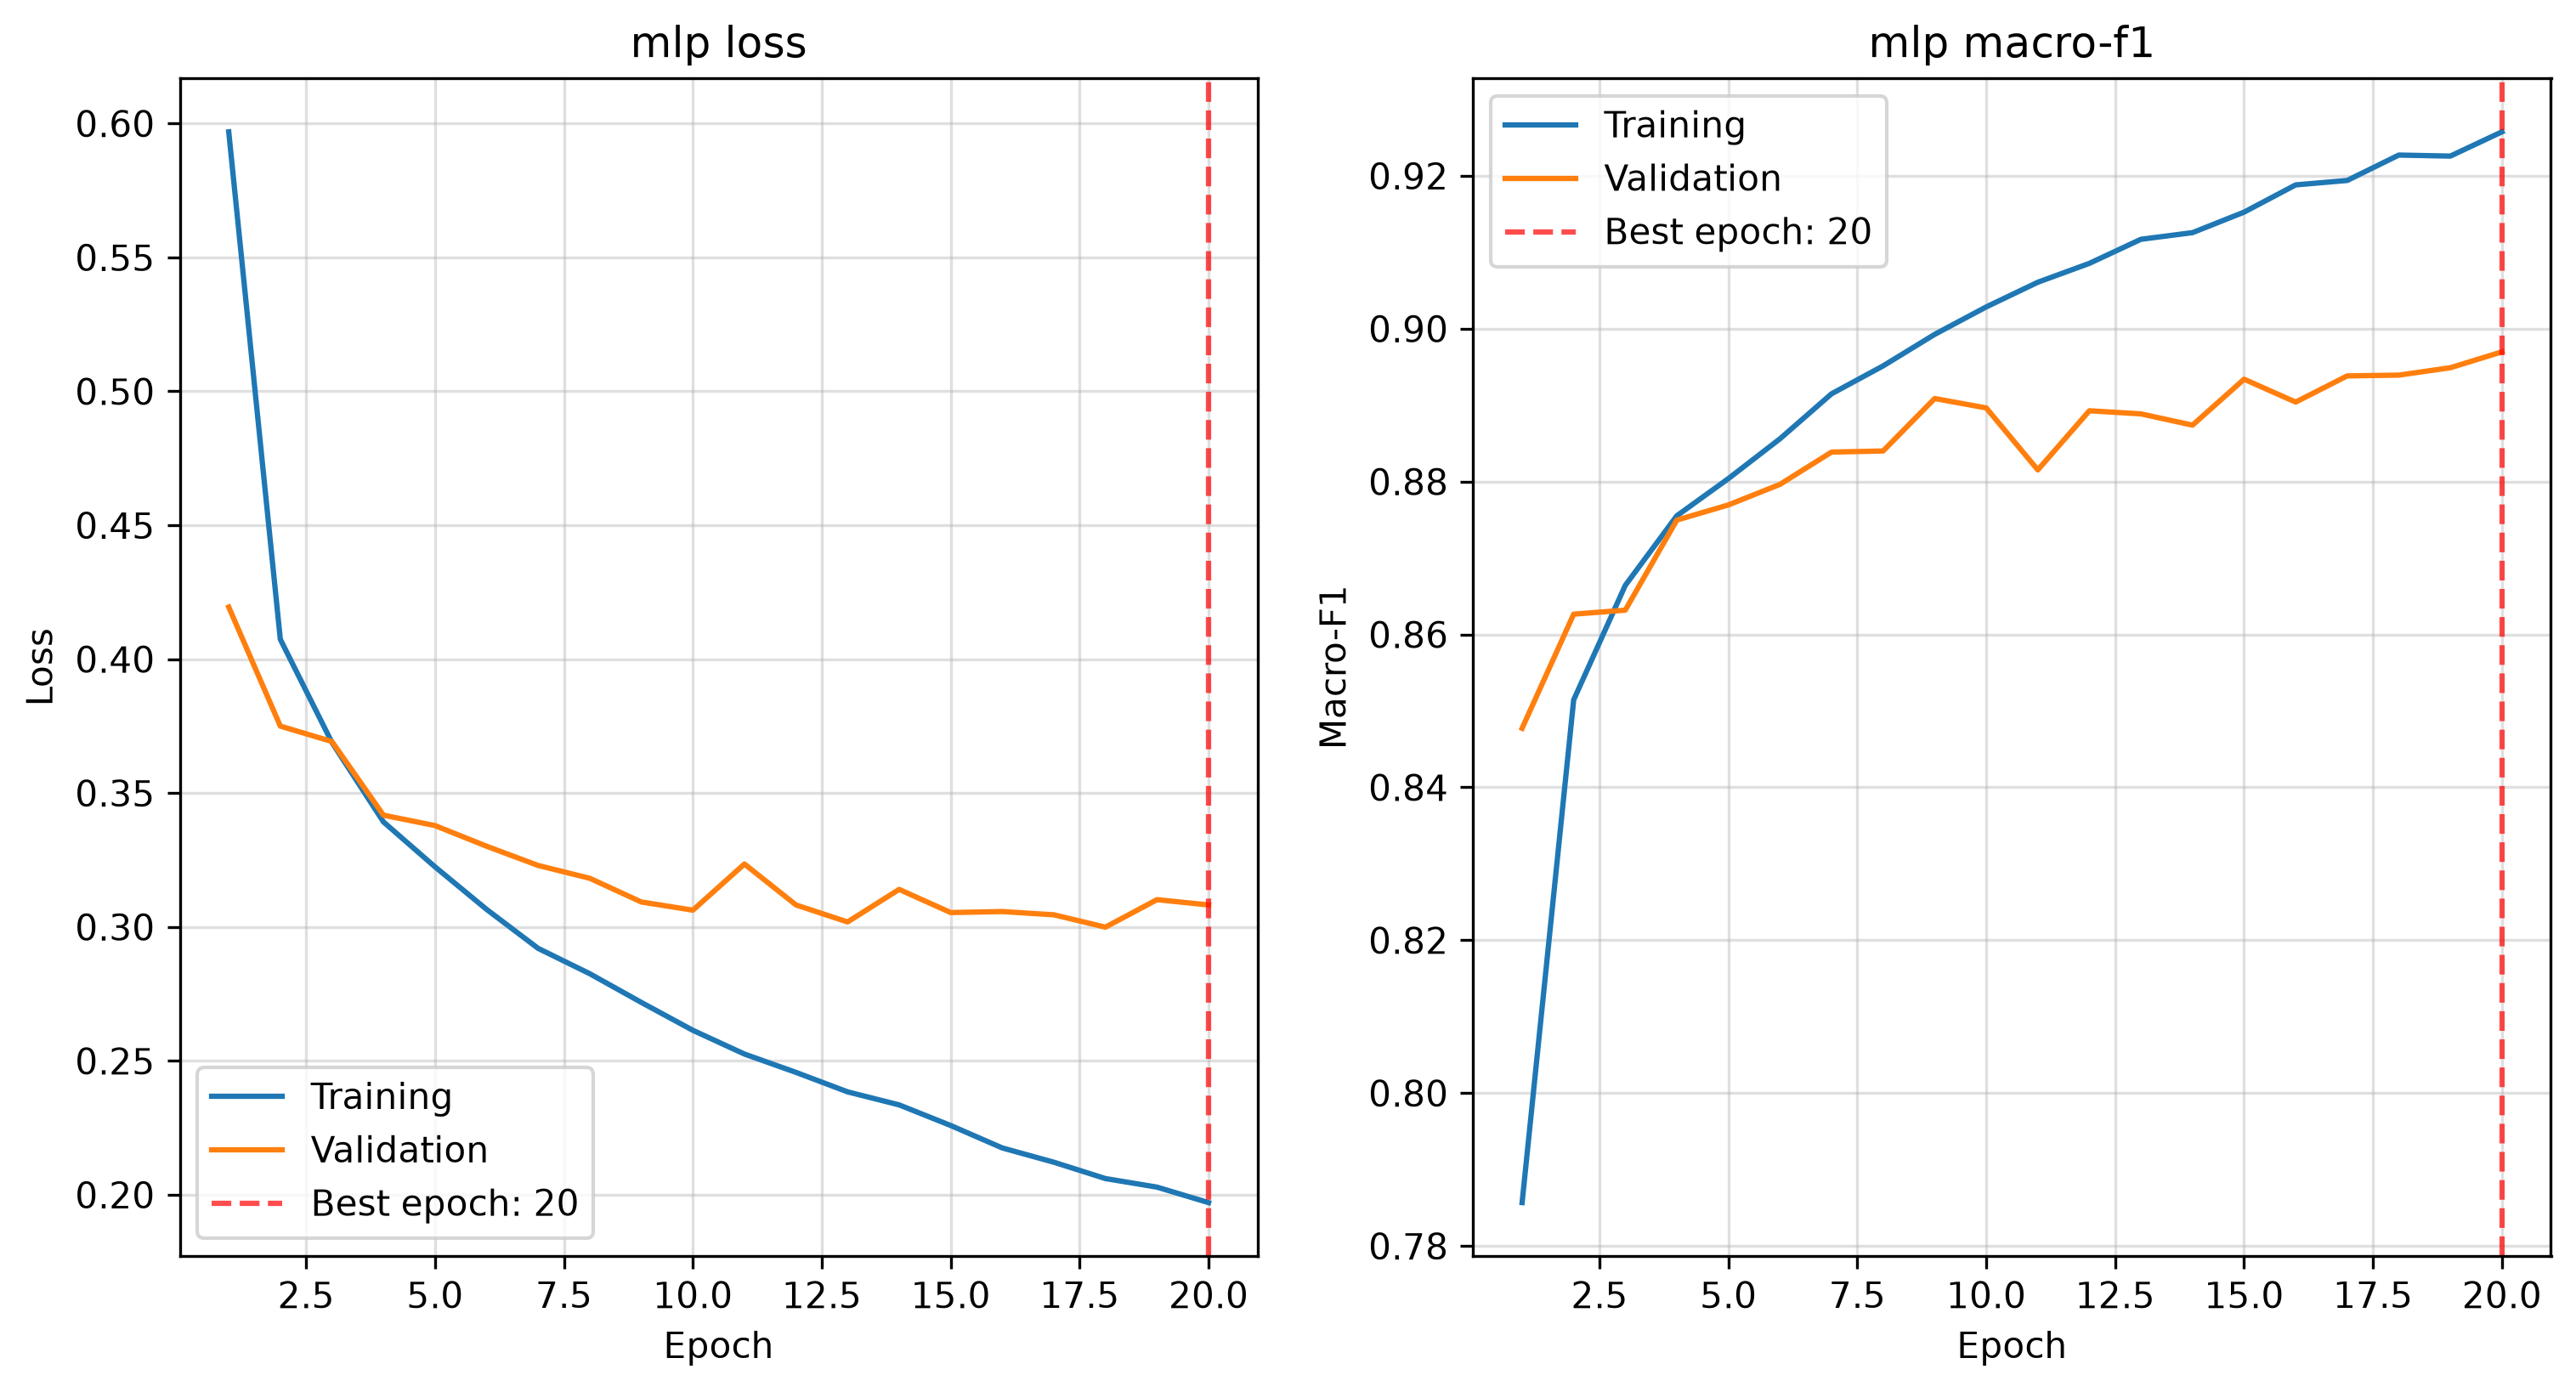
\includegraphics[width=\linewidth]{images/final_mlp_baseline_002_learning_curves.png}

\captionof{figure}{MLP: original training/validation loss and Macro-F1 curves from branch \texttt{a1}. The red dashed line marks the validation-selected epoch.}

\label{fig:learning-mlp}

\end{minipage}\par\medskip



\par\medskip\noindent\begin{minipage}{\linewidth}

\centering

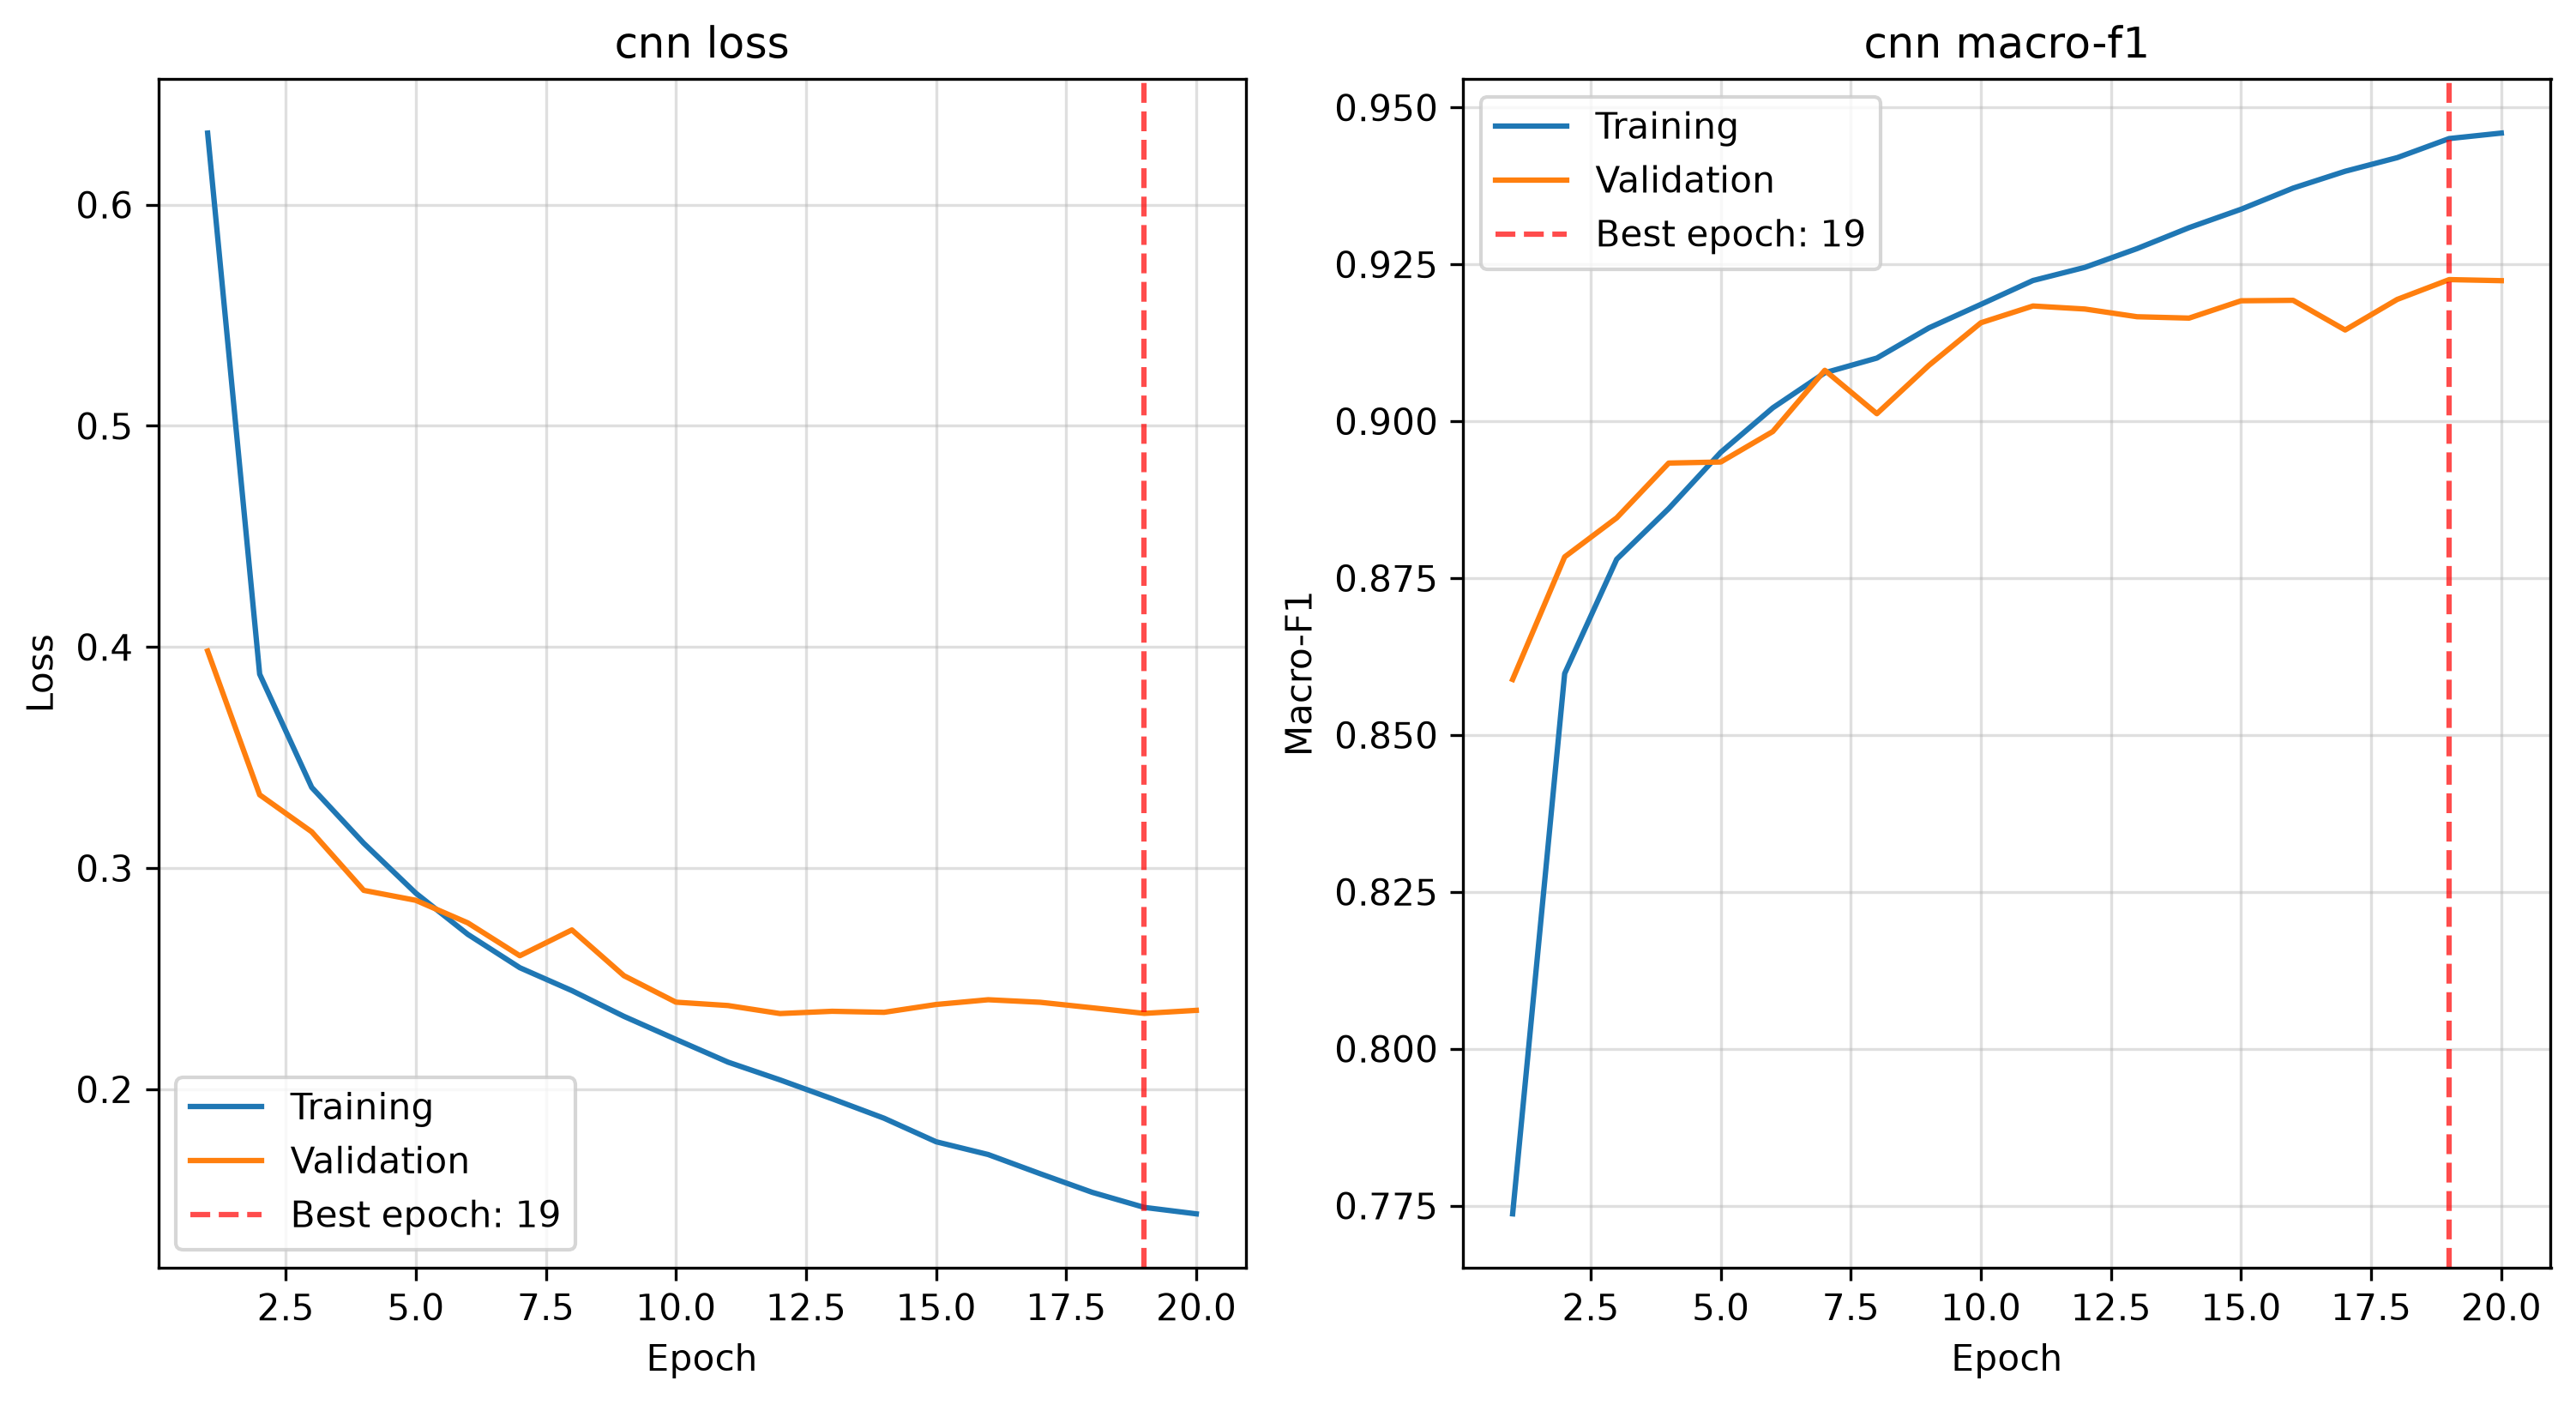
\includegraphics[width=\linewidth]{images/final_cnn_baseline_002_learning_curves.png}

\captionof{figure}{CNN: original training/validation loss and Macro-F1 curves from branch \texttt{a1}. The red dashed line marks the validation-selected epoch.}

\label{fig:learning-cnn}

\end{minipage}\par\medskip



\par\medskip\noindent\begin{minipage}{\linewidth}

\centering

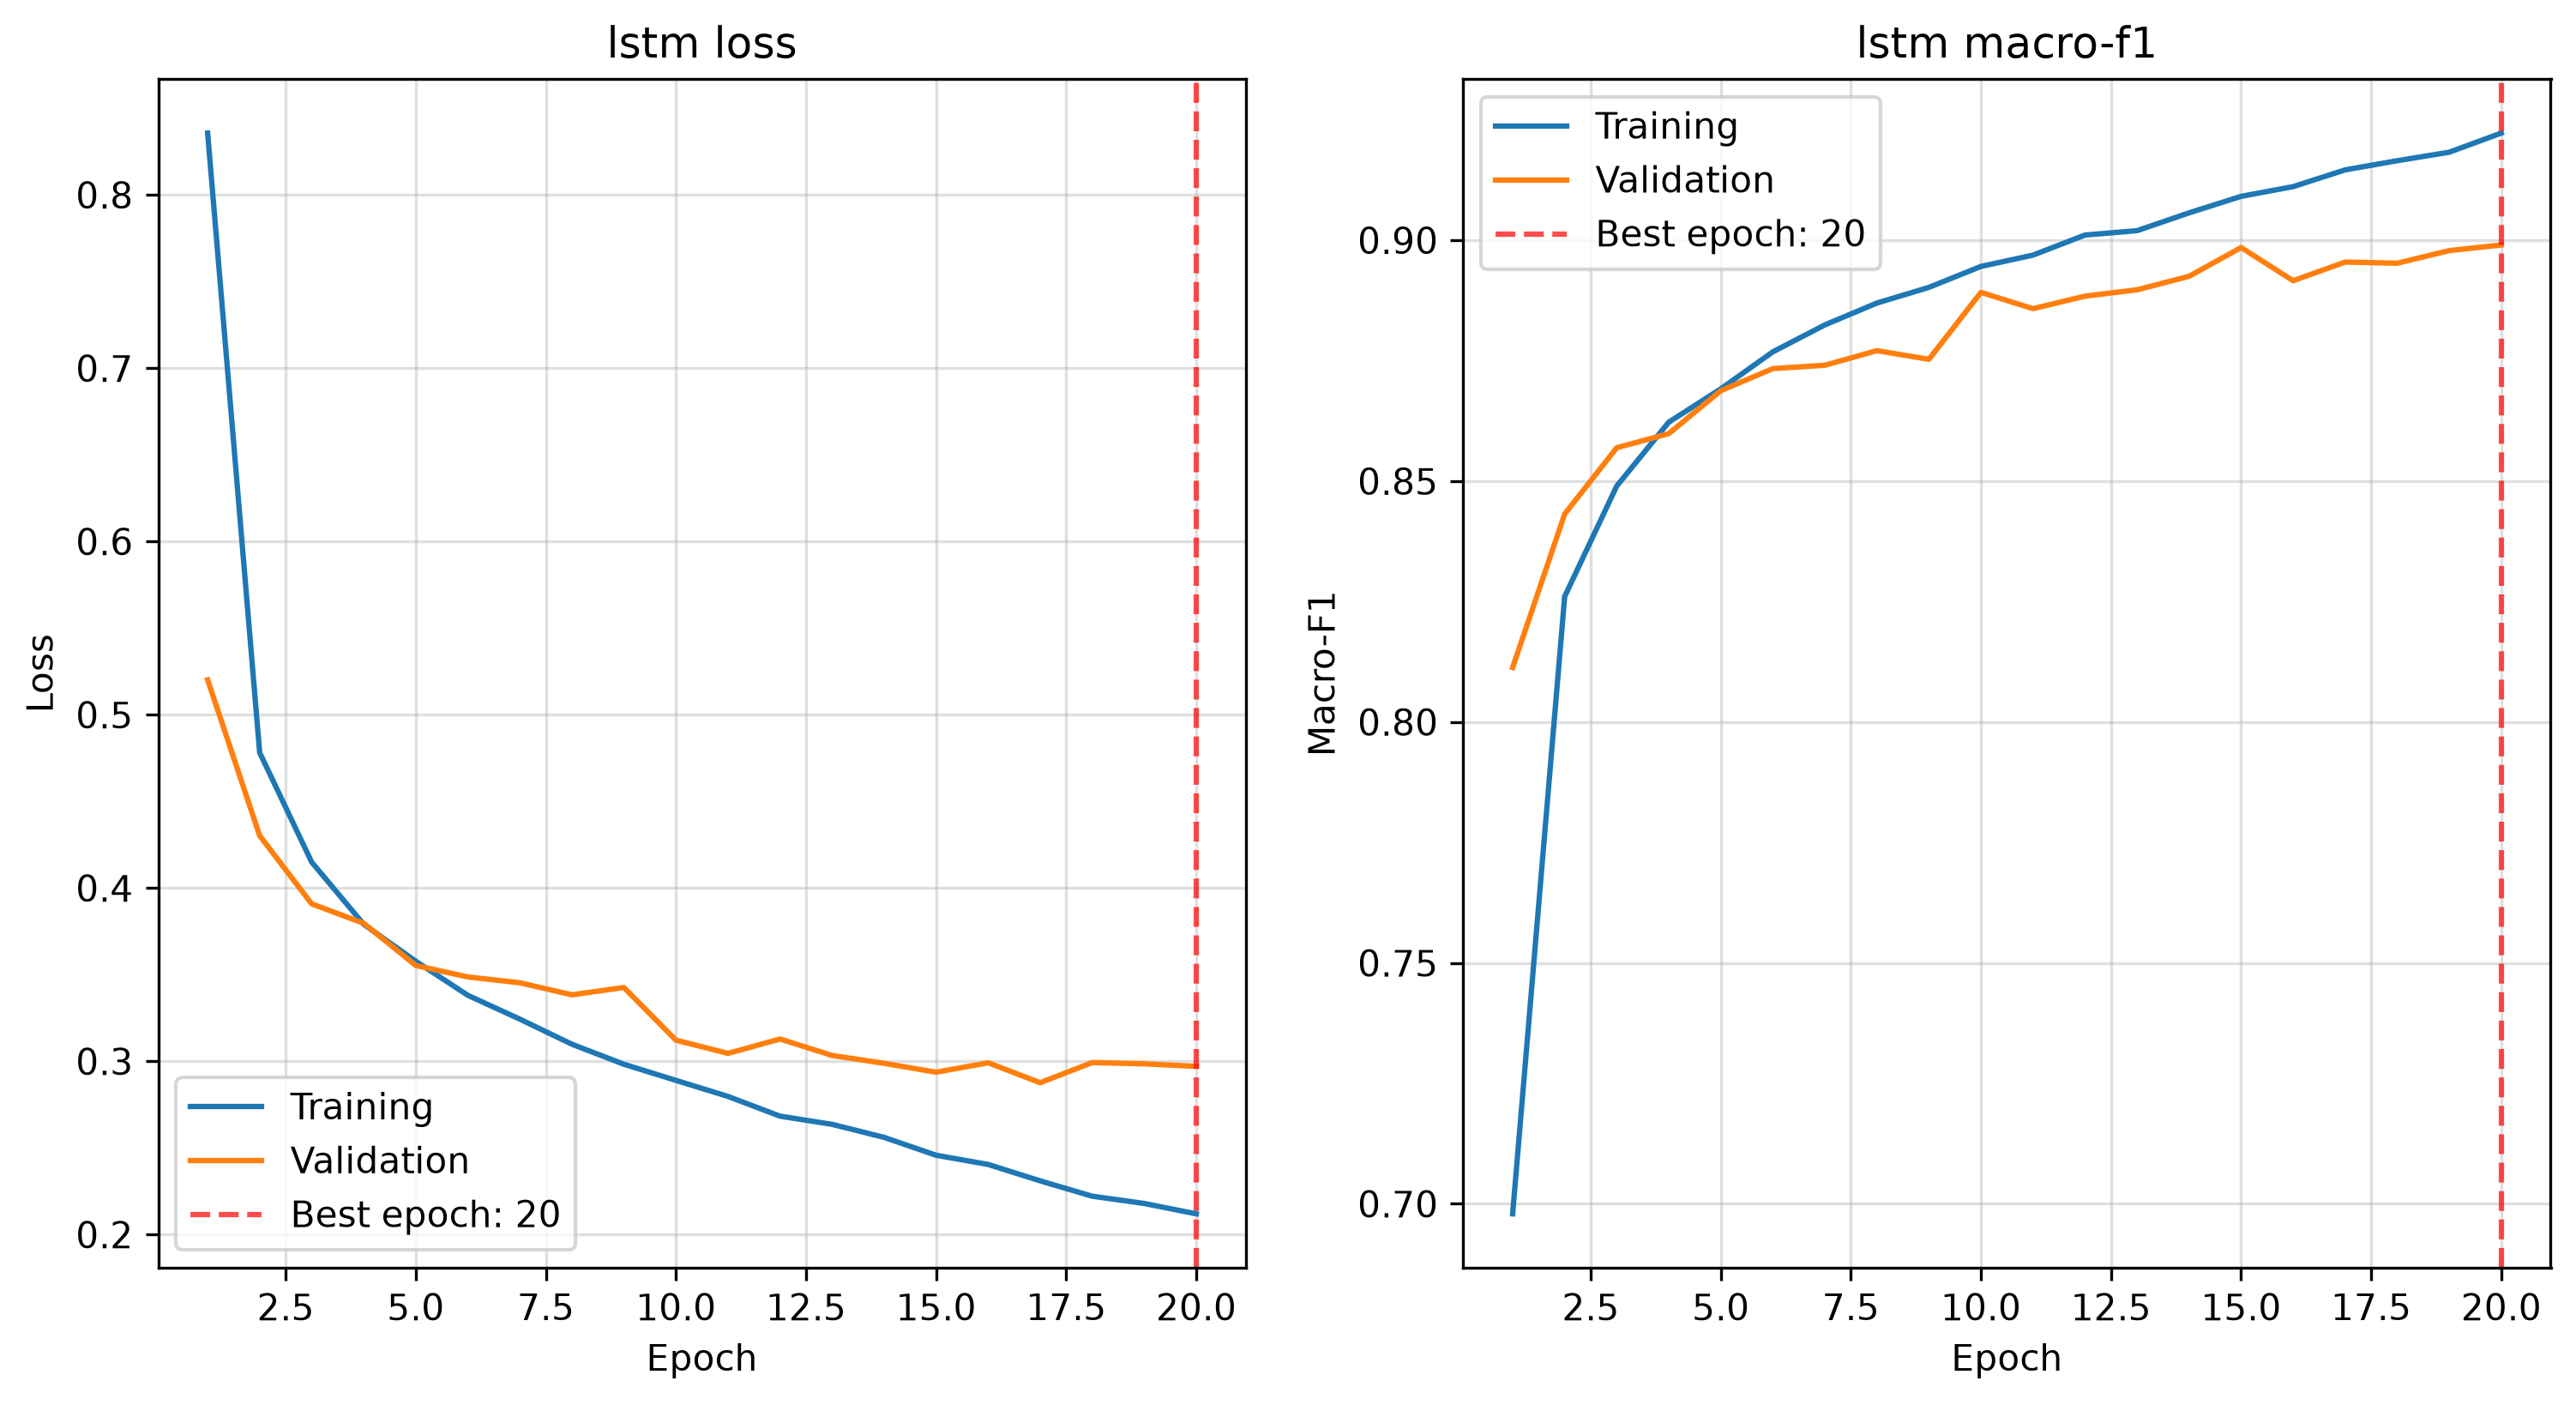
\includegraphics[width=\linewidth]{images/final_lstm_baseline_002_learning_curves.png}

\captionof{figure}{LSTM: original training/validation loss and Macro-F1 curves from branch \texttt{a1}. The red dashed line marks the validation-selected epoch.}

\label{fig:learning-lstm}

\end{minipage}\par\medskip



\par\medskip\noindent\begin{minipage}{\linewidth}

\centering

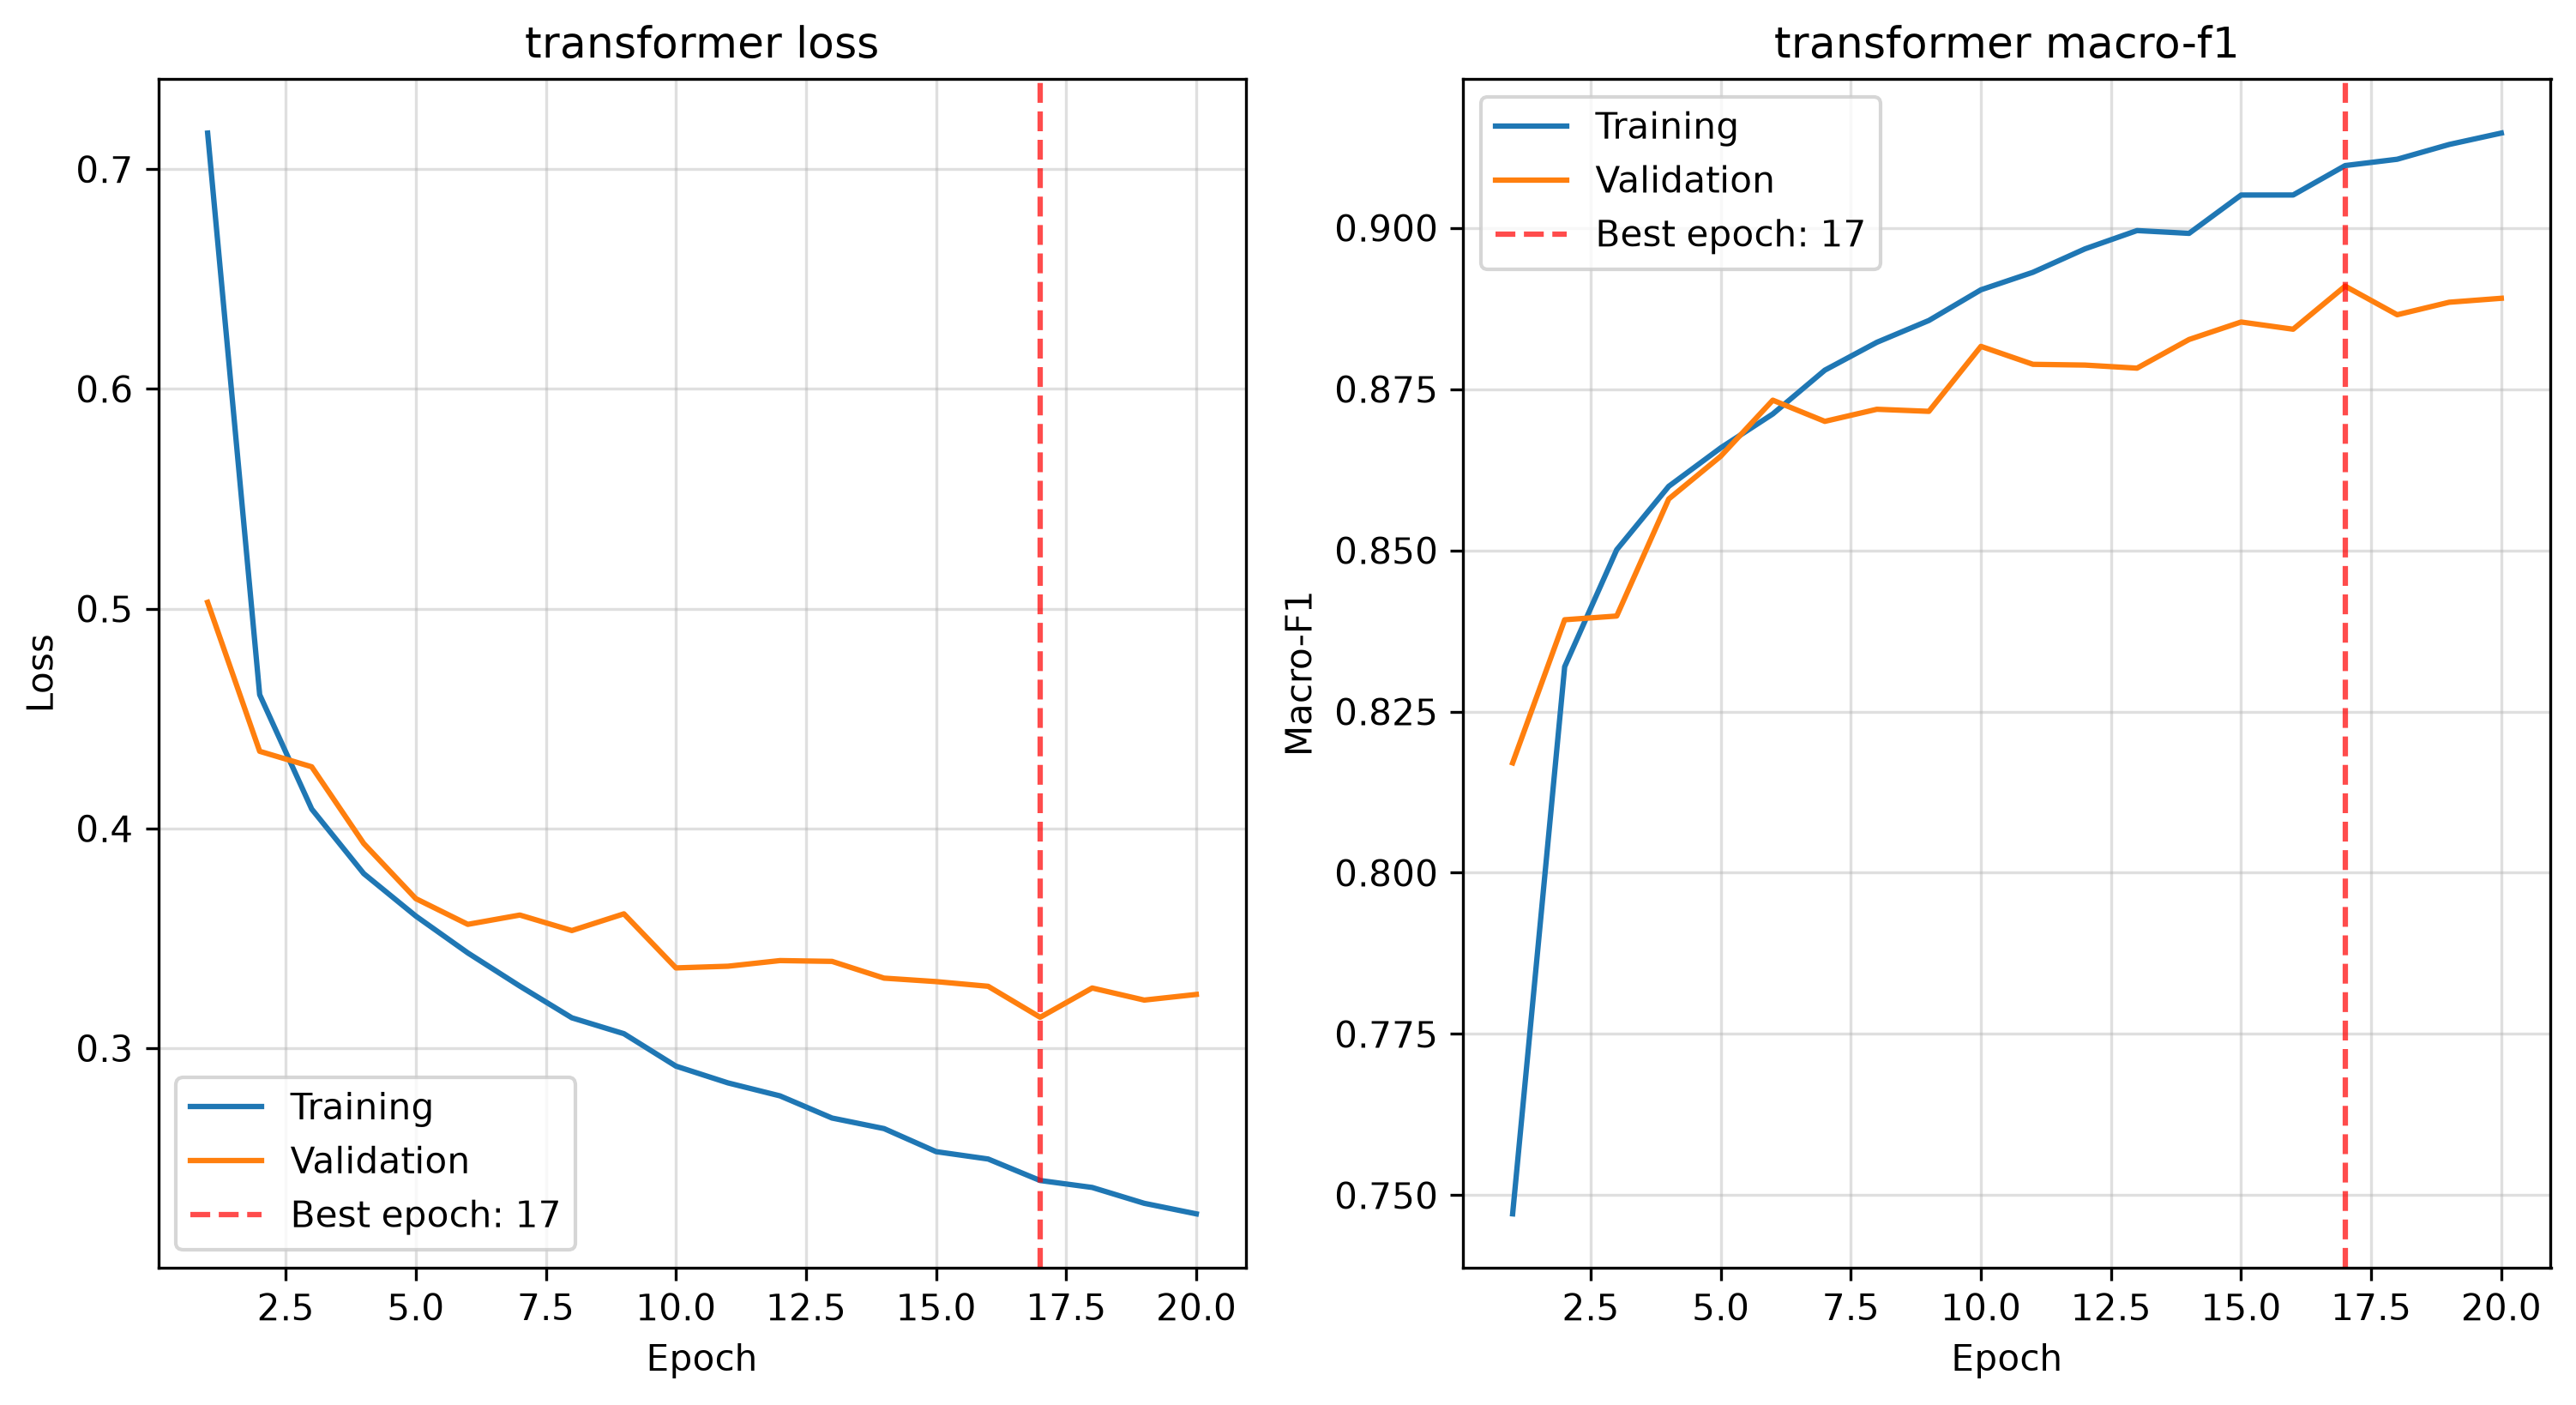
\includegraphics[width=\linewidth]{images/final_transformer_baseline_002_learning_curves.png}

\captionof{figure}{Transformer: original training/validation loss and Macro-F1 curves from branch \texttt{a1}. The red dashed line marks the validation-selected epoch.}

\label{fig:learning-transformer}

\end{minipage}\par\medskip



\subsubsection{Generalization Gaps}

\begin{itemize}
\setlength{\itemsep}{3pt}
\setlength{\parskip}{0pt}
\item \textbf{Accuracy gaps.} At epoch 20, train-minus-validation accuracy gaps are 1.45 percentage points (Linear), 2.97 (MLP), 2.46 (CNN), 2.35 (LSTM) and 2.64 (Transformer).
\item \textbf{Late-epoch behavior.} Training loss continues to improve while validation gains flatten, indicating limited late-epoch generalization gains under this budget.
\item \textbf{Interpretation.} The gaps alone do not prove a causal diagnosis of overfitting: training metrics include dropout and accumulate predictions while parameters change. Checkpoint selection limits the effect of late validation degradation.

\item \textbf{Traceability.} The branch contains all five model implementations, an inference benchmark, saved diagnostics and pytest-collected data-pipeline tests. The result records link each selected checkpoint to its configuration and metrics.
\end{itemize}


\subsection{Quantitative Comparison}

\subsubsection{Test Quality and Computational Cost}

\begin{table}[!htbp]\centering\small

\caption{Main five-model comparison: one seed, shared split and validation-based checkpoint selection. Inference is median CPU forward time per image.}

\label{tab:finalcomparison}

\begin{tabular}{@{}lrrrrr@{}}\toprule

Model & Acc. (\%) & Macro-F1 & Parameters & Train (s) & Infer. (ms)\\\midrule

CNN & 91.69 & 0.9163 & 220,234 & 1748.41 & 0.8216 \\

LSTM & 89.66 & 0.8960 & 214,282 & 1798.18 & 1.9652 \\

MLP & 89.08 & 0.8907 & 235,146 & 715.37 & 0.2037 \\

Transformer & 87.98 & 0.8790 & 274,954 & 2133.30 & 1.9598 \\

Linear & 84.31 & 0.8424 & 7,850 & 941.05 & 0.0484 \\

\bottomrule\end{tabular}\end{table}



\begin{itemize}
\setlength{\itemsep}{3pt}
\setlength{\parskip}{0pt}
\item \textbf{CNN.} It leads with 91.69\% Accuracy and 0.9163 Macro-F1, exceeding MLP by 2.61 percentage points and 0.0256 Macro-F1. Although it uses 6.34\% fewer parameters than MLP, training takes about 2.44 times longer and median inference about 4.03 times longer. It provides the highest observed quality at a higher computational cost than MLP.
\item \textbf{MLP.} It achieves 89.08\% Accuracy and 0.8907 Macro-F1. It has the lowest recorded training time (715.37 s) and a median inference time of 0.2037 ms/image, approximately one quarter of CNN's. These measurements make it a useful quality--latency compromise on the recorded CPU; timing cannot be inferred from parameter count alone.
\item \textbf{LSTM.} It ranks second at 89.66\% Accuracy and 0.8960 Macro-F1. Its gain over MLP is 0.58 percentage points and 0.0053 Macro-F1, while median inference takes about 9.64 times longer. The modest quality gain therefore comes with a substantial latency cost.
\item \textbf{Transformer.} It reaches 87.98\% Accuracy and 0.8790 Macro-F1, trailing MLP by 1.10 percentage points. It also has the largest parameter count (274,954) and longest recorded training time (2,133.30 s). Its greater architectural flexibility does not improve the quality--cost trade-off under this configuration and budget.
\item \textbf{Linear.} It reaches 84.31\% Accuracy and 0.8424 Macro-F1, the lowest scores among the five models. With 7,850 parameters and a median inference time of 0.0484 ms/image, it is the smallest and fastest model. It offers the lowest forward cost but sacrifices classification quality.
\end{itemize}






\subsubsection{Timing Resolution and Single-Seed Uncertainty}

\begin{itemize}
\setlength{\itemsep}{3pt}
\setlength{\parskip}{0pt}
\item \textbf{Timing spread.} Stored p95 forward times are 0.0570 ms (Linear), 0.2323 (MLP), 0.9844 (CNN), 2.5340 (LSTM) and 2.1620 (Transformer).
\item \textbf{Close medians.} LSTM and Transformer have almost equal medians (1.9652 and 1.9598 ms); their tiny median difference is not a reliable speed distinction from only 20 repeated passes.
\item \textbf{Measurement limits.} CPU scheduling, thread behavior and kernel implementations influence these values. Training times also include validation and checkpoint overhead.

\item \textbf{Single-seed scope.} The reported scores are single-seed measurements. No multi-seed mean, standard deviation or significance claim is supported.
\item \textbf{Limits of comparison.} In particular, the modest LSTM--MLP gap should be treated as an observation for these saved runs. Different run-number suffixes do not provide independent seed replications.
\end{itemize}


\subsection{Per-Class and Qualitative Results}

\subsubsection{Confusion Matrices and Class-Wise F1}

\begin{itemize}
\setlength{\itemsep}{3pt}
\setlength{\parskip}{0pt}
\item \textbf{Confusion matrices.} Figures~\ref{fig:confusions}--\ref{fig:confusions-transformer} reproduce the original row-normalized confusion matrices for all five models.
\item \textbf{Per-class evaluation.} Table~\ref{tab:perclass} provides per-class F1; each class has exactly 1,000 test examples. High aggregate accuracy does not remove the much larger error rate on Shirt.
\end{itemize}
\par\medskip\noindent\begin{minipage}{\linewidth}\centering\small

\captionof{table}{Per-class F1 from the committed error-analysis JSON files. Values are rounded to three decimals; the macro scores use unrounded values.}

\label{tab:perclass}

\begin{tabular}{@{}lrrrrr@{}}\toprule

Class & Linear & MLP & CNN & LSTM & Transformer\\\midrule

T-shirt/top & 0.809 & 0.851 & 0.865 & 0.847 & 0.828\\

Trouser & 0.969 & 0.980 & 0.984 & 0.977 & 0.975\\

Pullover & 0.725 & 0.816 & 0.872 & 0.830 & 0.792\\

Dress & 0.854 & 0.895 & 0.914 & 0.895 & 0.889\\

Coat & 0.749 & 0.813 & 0.871 & 0.822 & 0.805\\

Sandal & 0.930 & 0.965 & 0.983 & 0.970 & 0.962\\

Shirt & 0.592 & 0.710 & 0.753 & 0.717 & 0.672\\

Sneaker & 0.922 & 0.950 & 0.964 & 0.958 & 0.944\\

Bag & 0.933 & 0.974 & 0.986 & 0.976 & 0.965\\

Ankle boot & 0.943 & 0.954 & 0.971 & 0.968 & 0.957\\

\bottomrule\end{tabular}\end{minipage}\par\medskip



\begin{itemize}
\setlength{\itemsep}{3pt}
\setlength{\parskip}{0pt}
\item \textbf{Hardest class.} Shirt is the weakest class for every model. CNN improves its F1 from Linear's 0.592 to 0.753, but its recall is still only 71.2\%: 288 of 1,000 shirts are missed.
\item \textbf{Strong classes.} CNN's best class is Bag (F1 0.986), with 98.7\% recall. Trouser and Sandal are also strong (F1 about 0.984).
\item \textbf{Uneven gains.} The CNN does not lead every class: LSTM has slightly higher Trouser recall (97.4\% versus 97.3\%), although CNN's precision gives it the higher F1. The gains are uneven across classes. Overall Macro-F1 is determined by the average across all ten classes, not a single easy category.
\end{itemize}


\par\medskip\noindent\begin{minipage}{\linewidth}

\centering

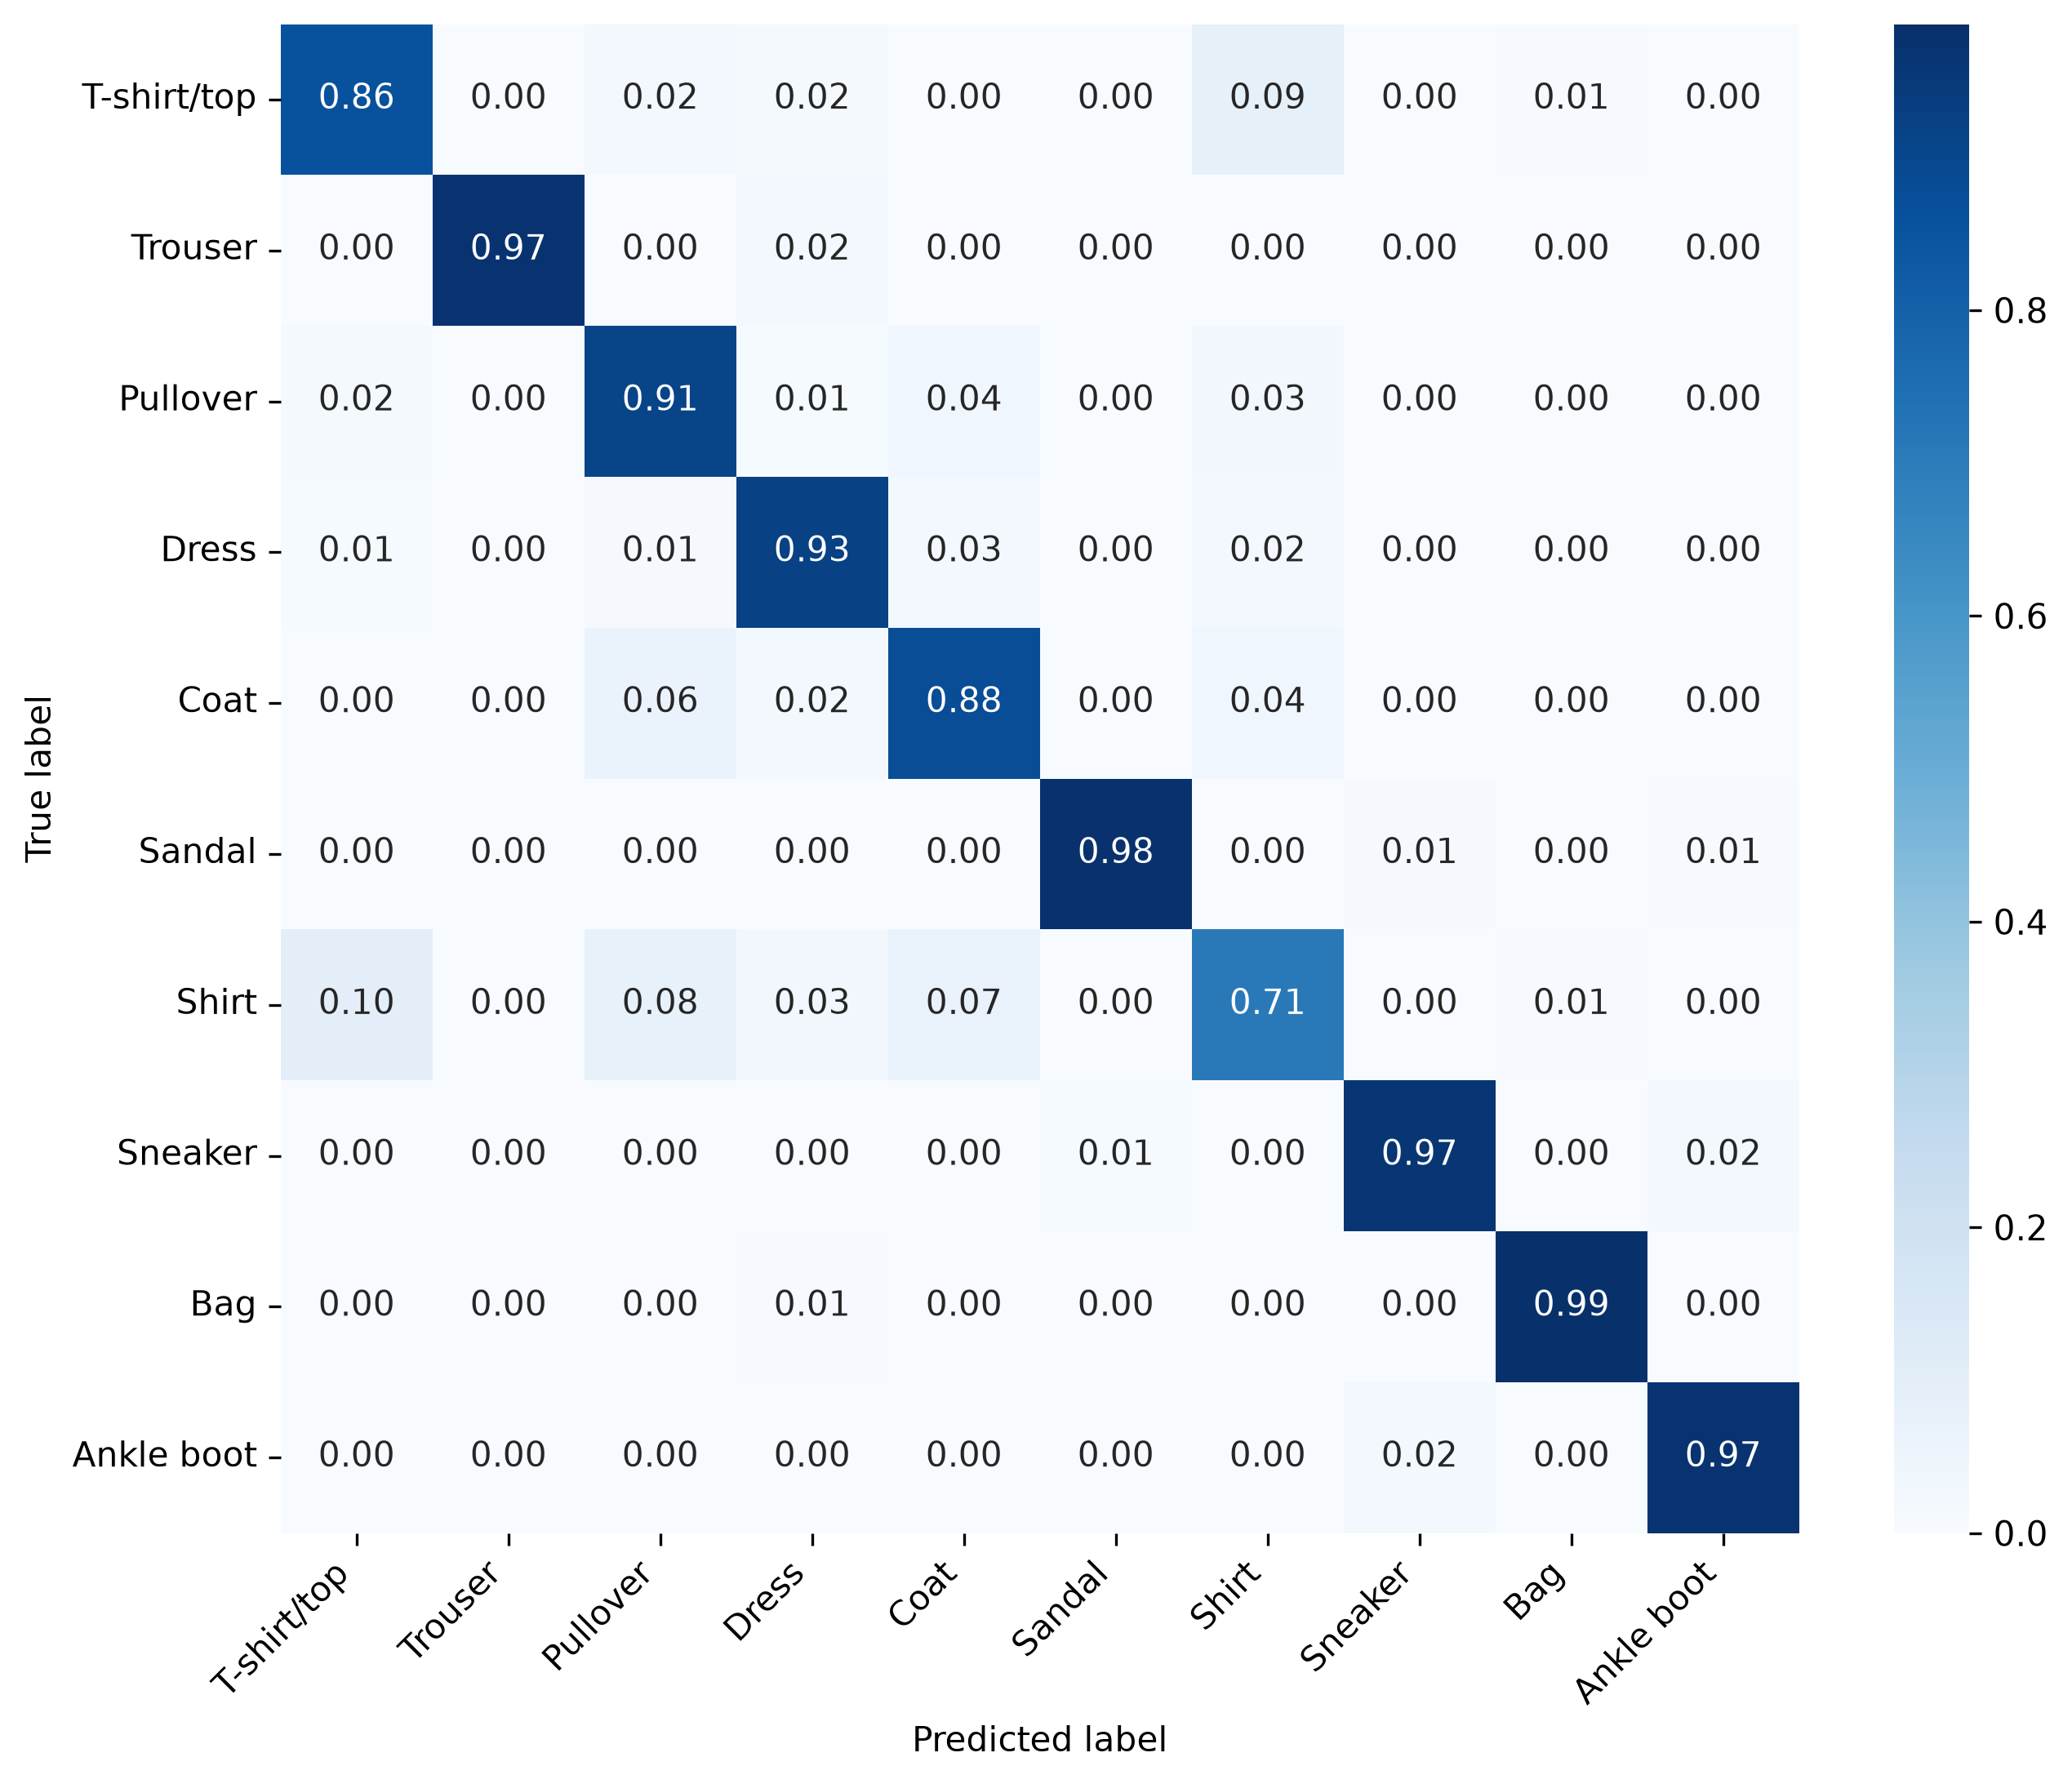
\includegraphics[width=.84\linewidth]{images/final_cnn_cm_normalized.png}

\captionof{figure}{Original CNN confusion matrix from branch \texttt{a1}. Rows are true labels, columns are predictions and entries are row-normalized. Table~\ref{tab:cnnerrors} reports the largest directed error counts.}

\label{fig:confusions}

\end{minipage}\par\medskip



\par\medskip\noindent\begin{minipage}{\linewidth}
\centering
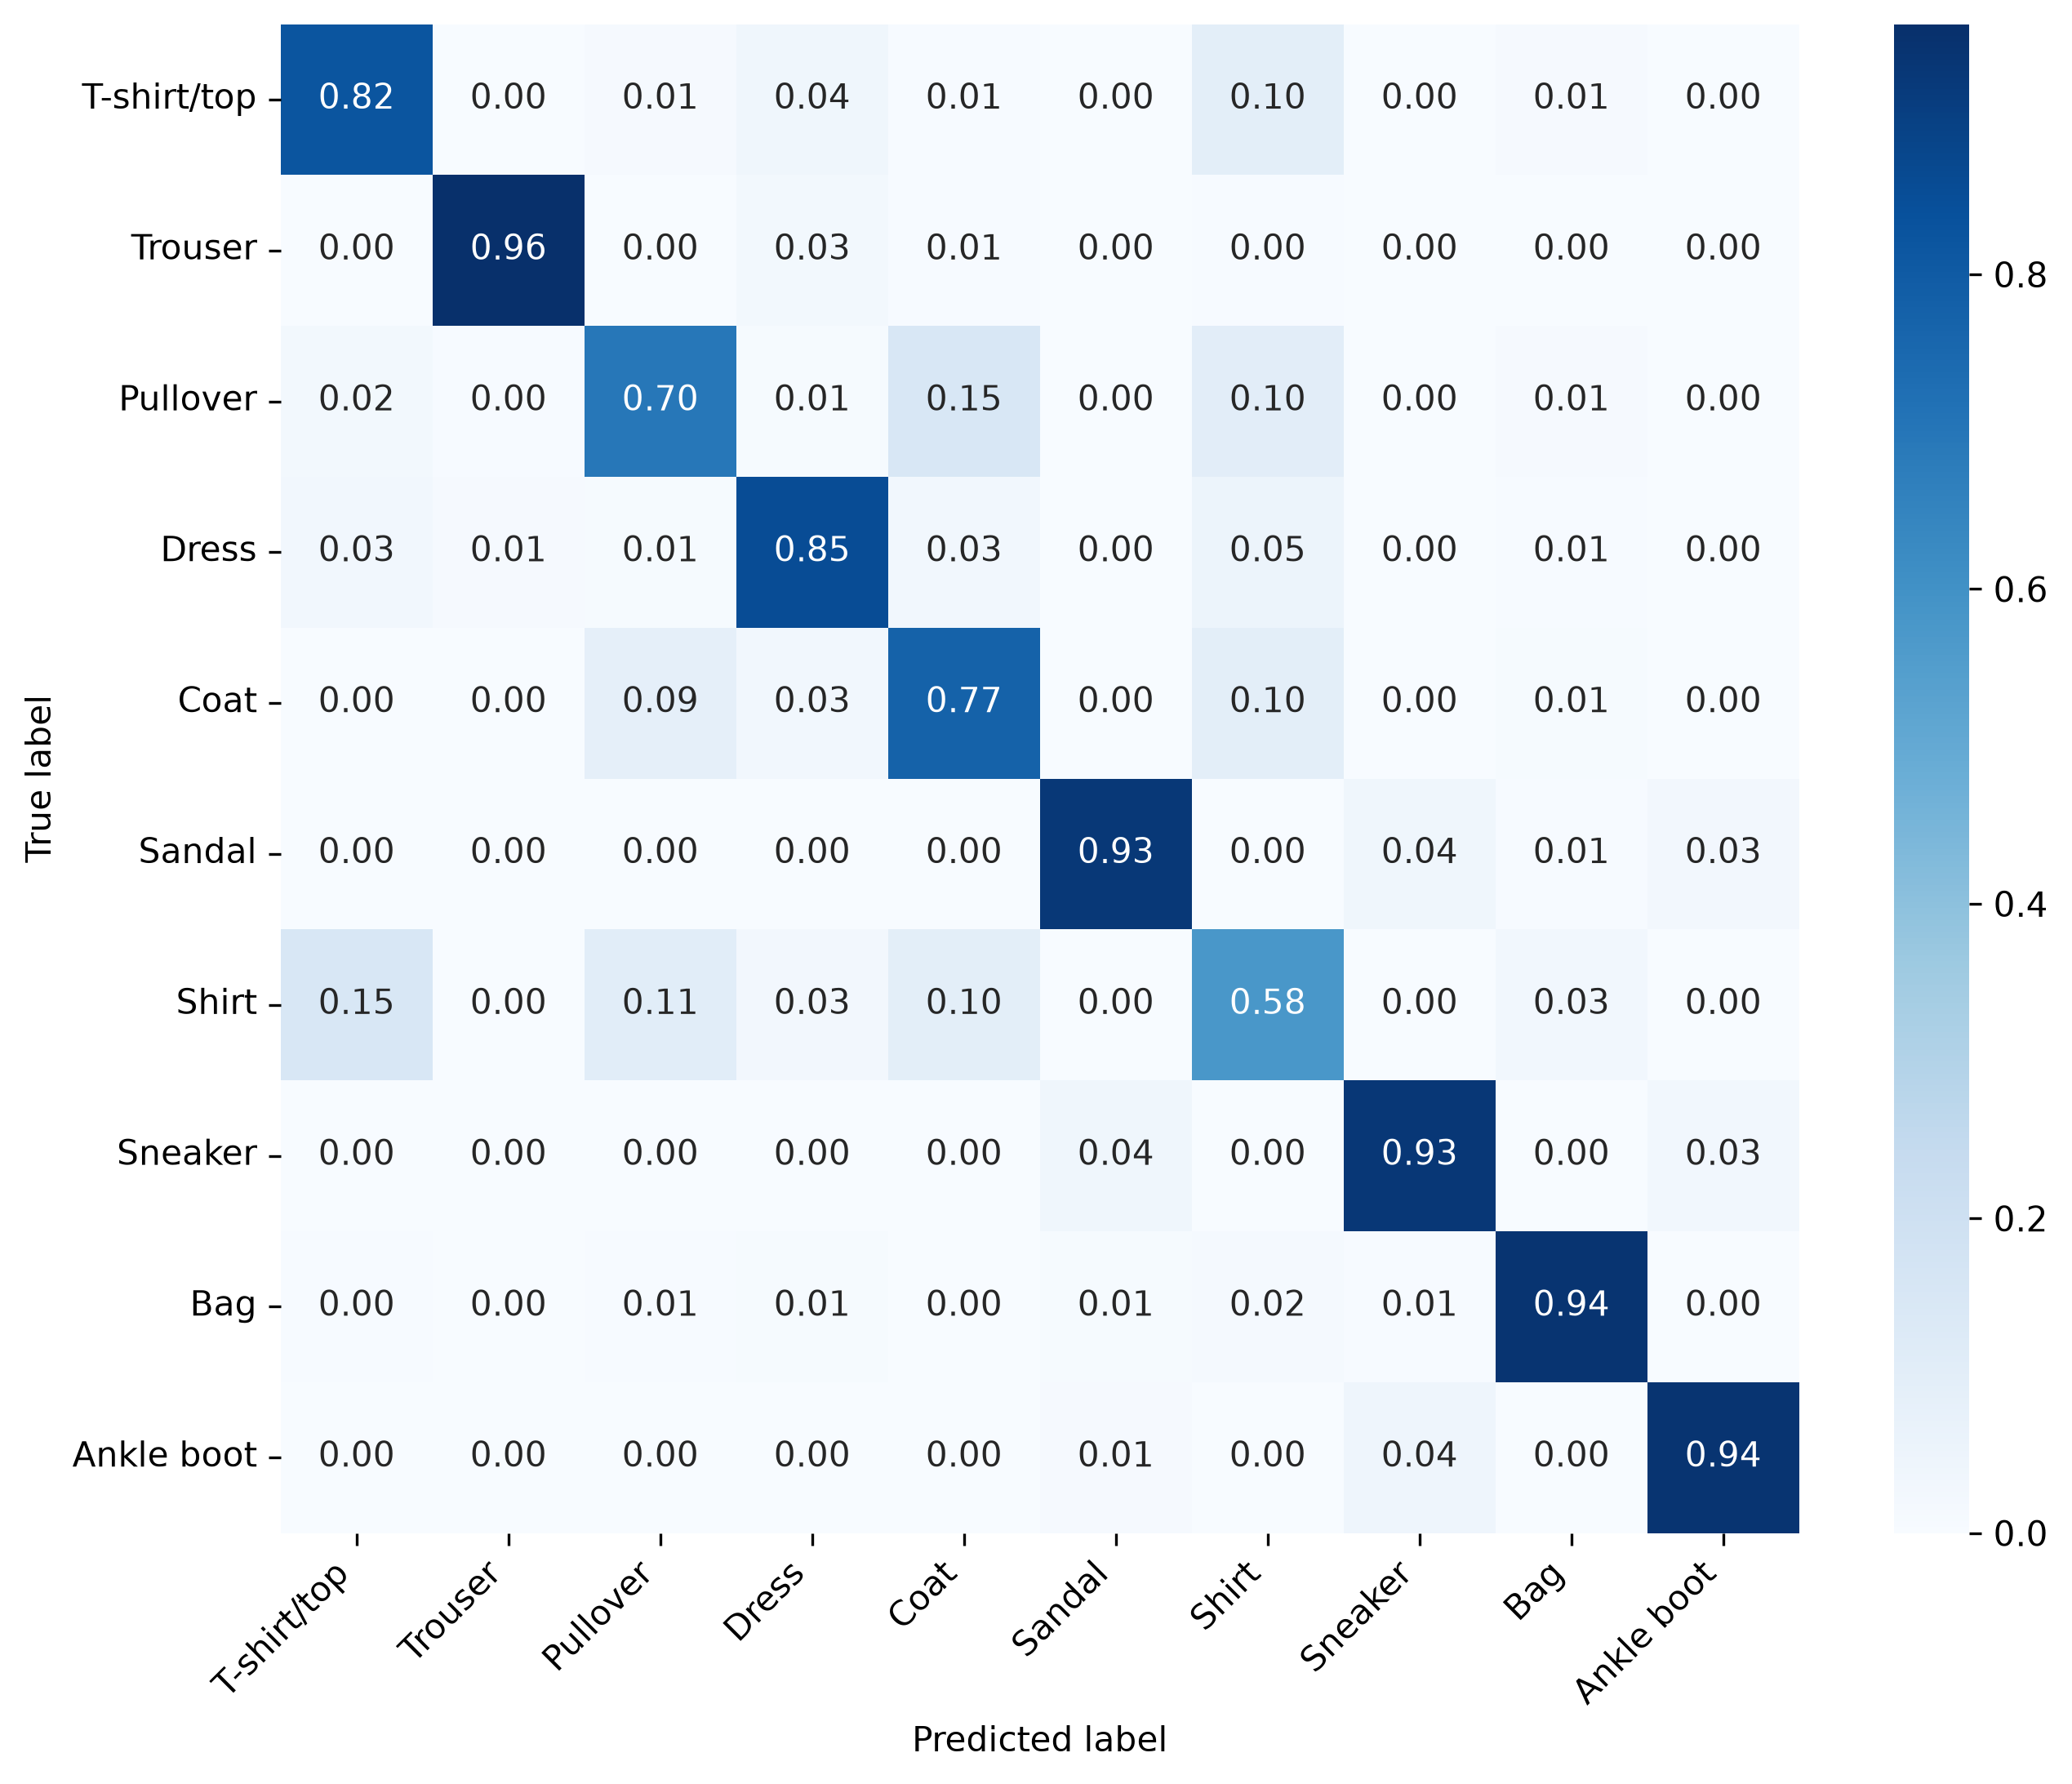
\includegraphics[width=.84\linewidth,height=.40\textheight,keepaspectratio]{images/final_linear_cm_normalized.png}
\captionof{figure}{Linear: original row-normalized confusion matrix from the selected branch run.}
\label{fig:confusions-linear}
\end{minipage}\par\medskip

\par\medskip\noindent\begin{minipage}{\linewidth}
\centering
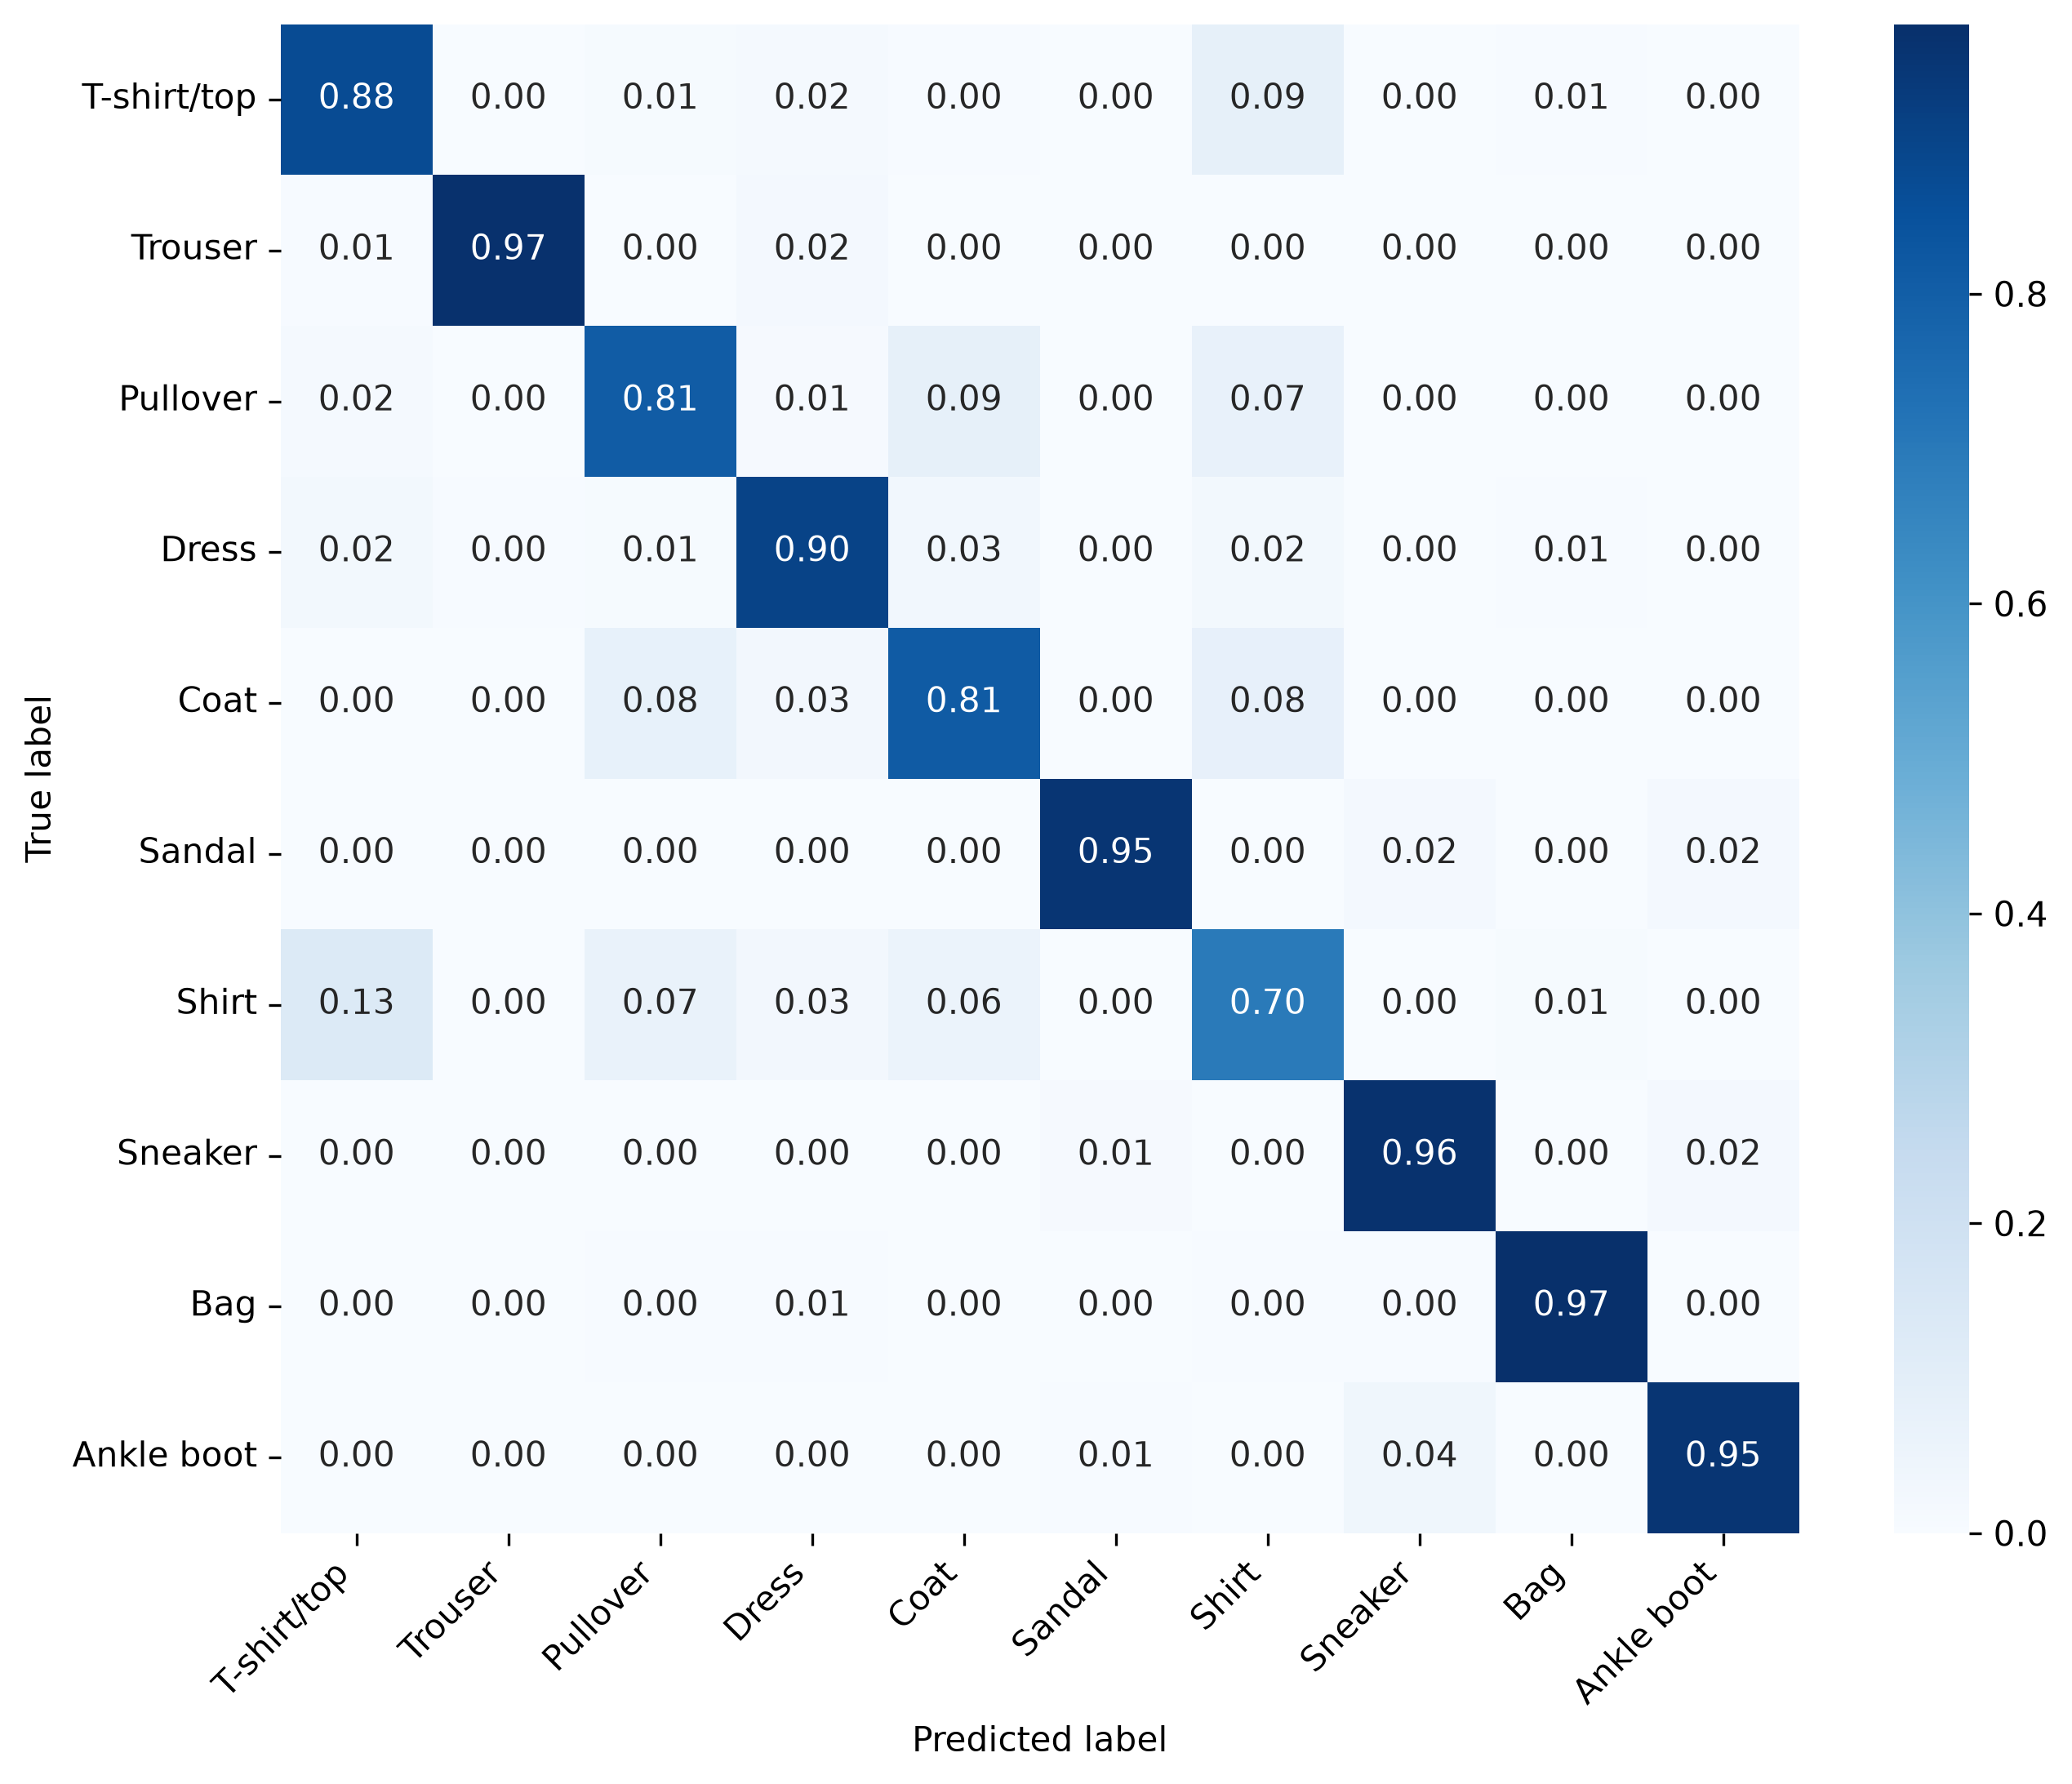
\includegraphics[width=.84\linewidth,height=.40\textheight,keepaspectratio]{images/final_mlp_cm_normalized.png}
\captionof{figure}{MLP: original row-normalized confusion matrix from the selected branch run.}
\label{fig:confusions-mlp}
\end{minipage}\par\medskip

\par\medskip\noindent\begin{minipage}{\linewidth}
\centering
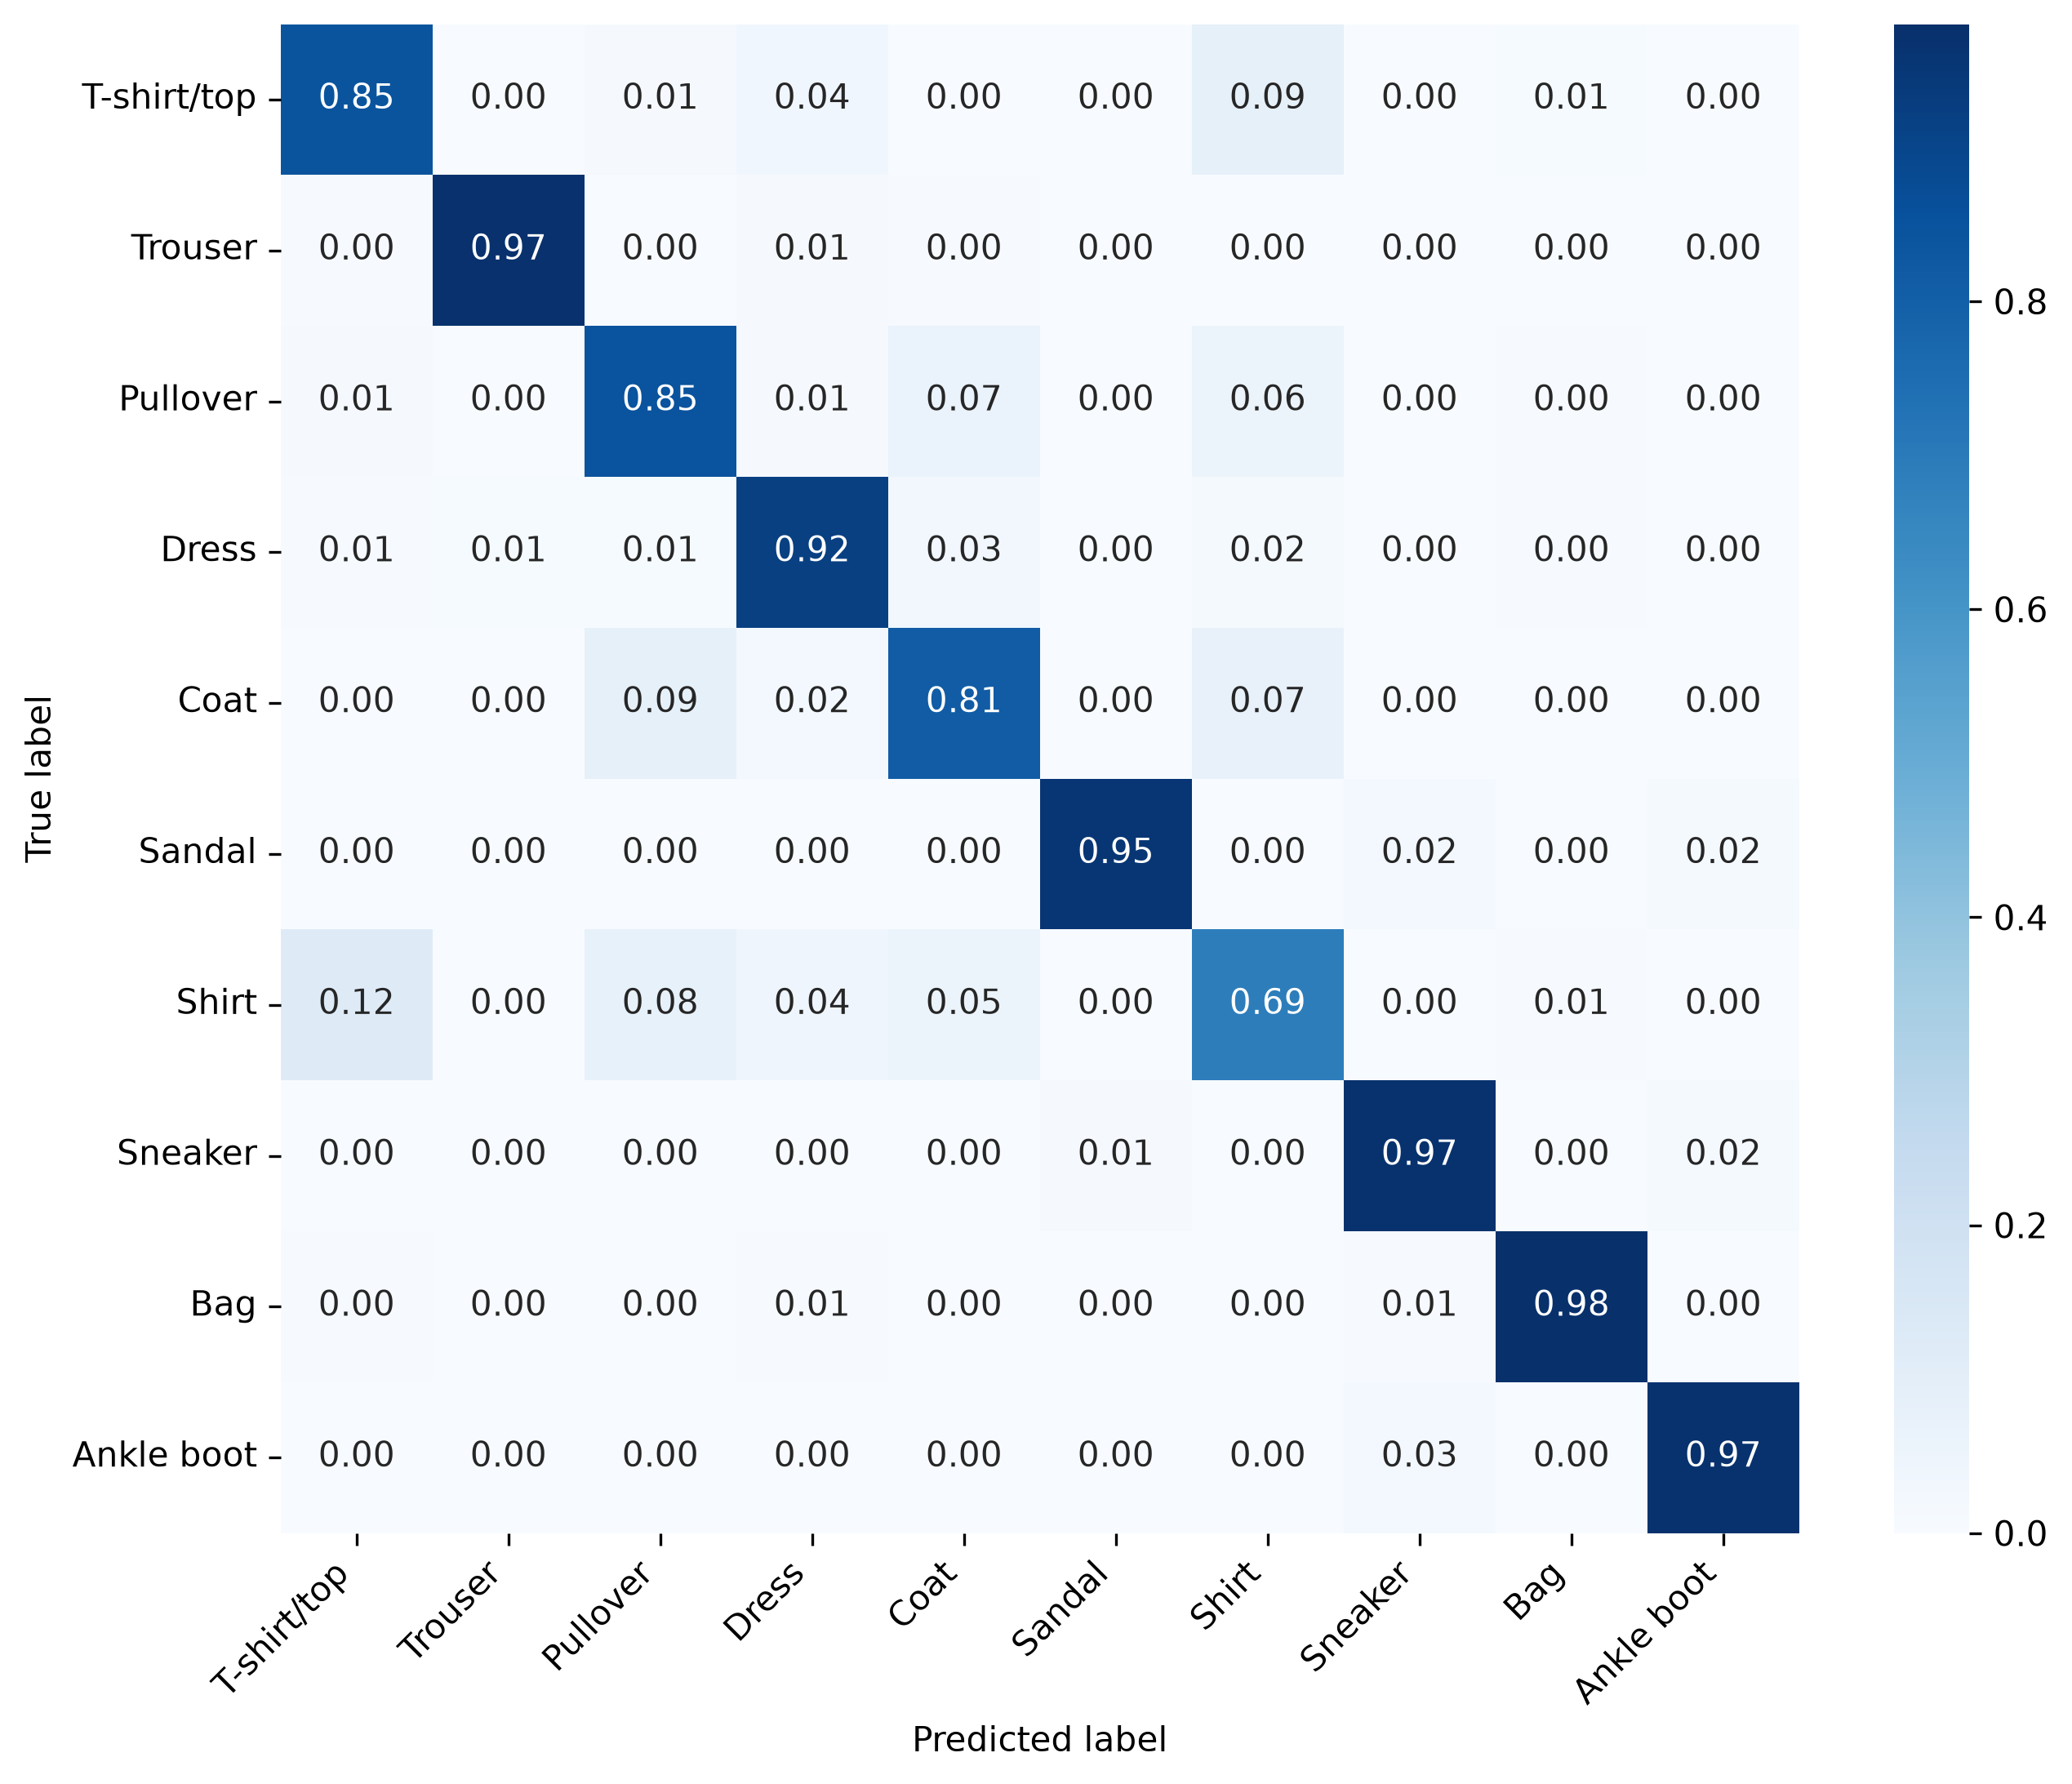
\includegraphics[width=.84\linewidth,height=.40\textheight,keepaspectratio]{images/final_lstm_cm_normalized.png}
\captionof{figure}{LSTM: original row-normalized confusion matrix from the selected branch run.}
\label{fig:confusions-lstm}
\end{minipage}\par\medskip

\par\medskip\noindent\begin{minipage}{\linewidth}
\centering
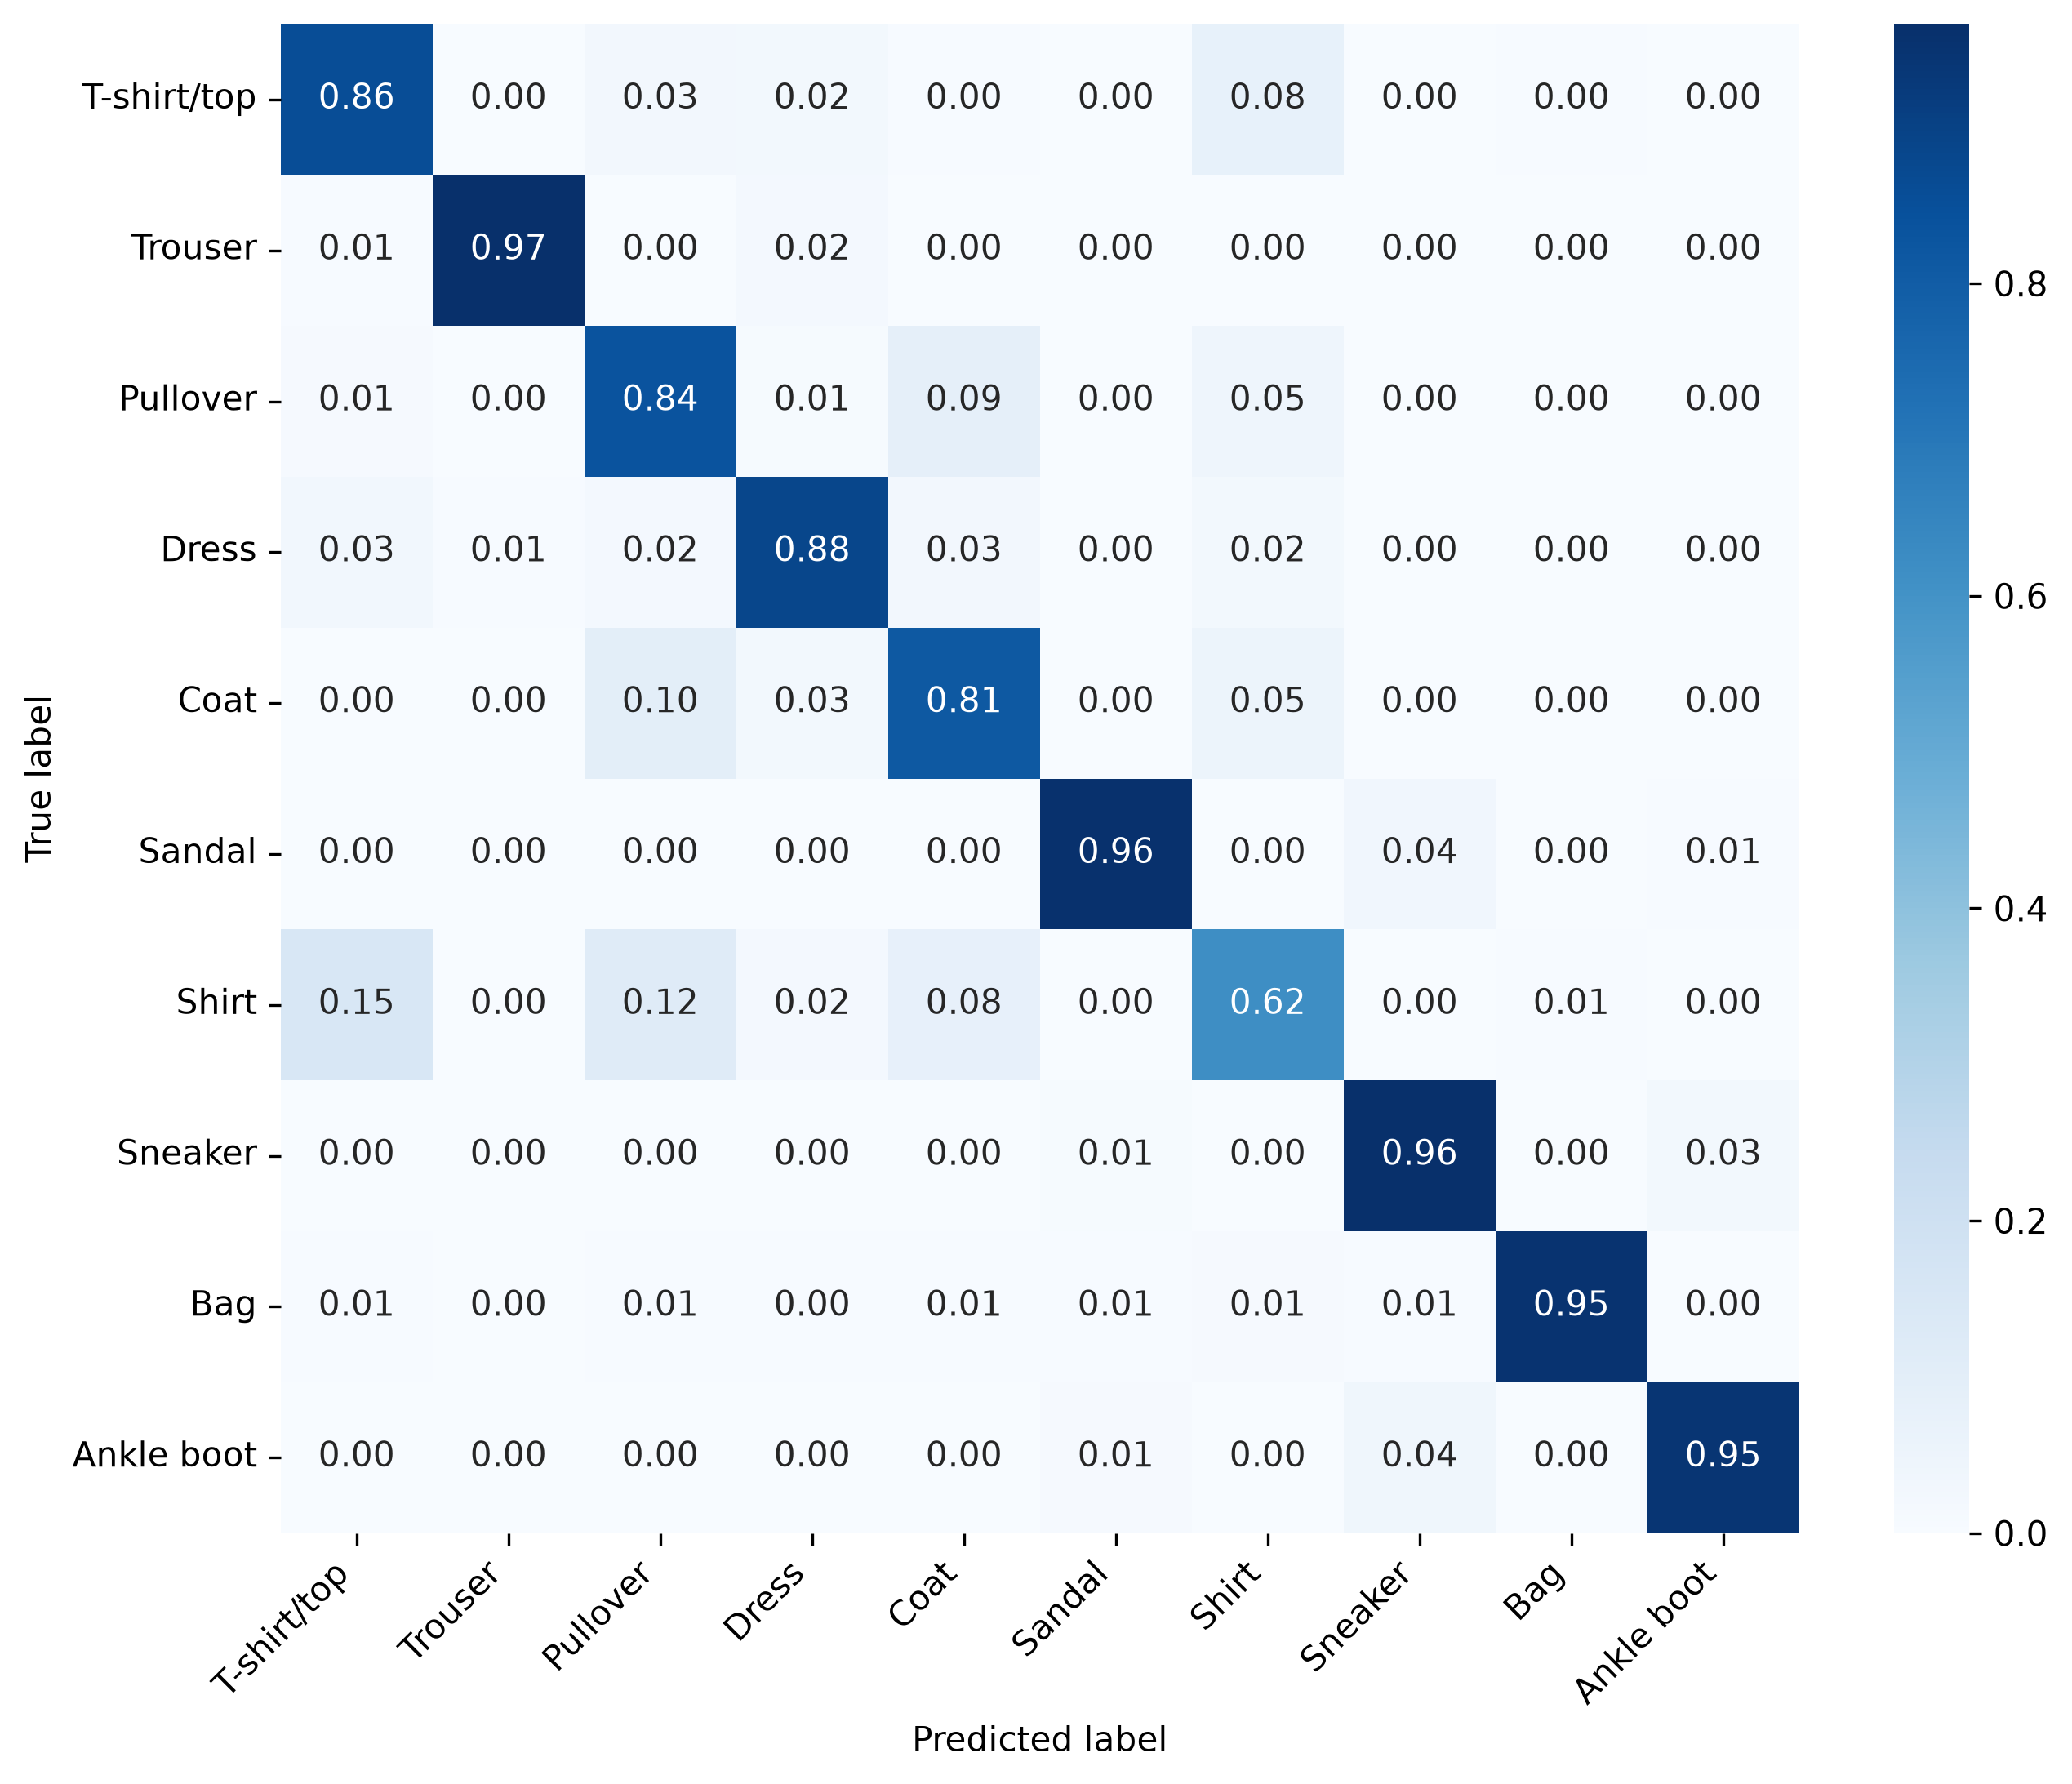
\includegraphics[width=.84\linewidth,height=.40\textheight,keepaspectratio]{images/final_transformer_cm_normalized.png}
\captionof{figure}{Transformer: original row-normalized confusion matrix from the selected branch run.}
\label{fig:confusions-transformer}
\end{minipage}\par\medskip

\subsubsection{Correct and Incorrect Prediction Examples}

\begin{itemize}
\setlength{\itemsep}{3pt}
\setlength{\parskip}{0pt}
\item \textbf{Correct predictions.} Figure~\ref{fig:cnnexamples} reproduces five correct and five incorrect CNN predictions from the branch. The correctly recognized Pullover contains visible internal structure despite its coarse resolution; the Ankle boot has a recognizable silhouette.
\item \textbf{Failure examples.} The incorrect Sneaker-to-Bag and Ankle-boot-to-Sandal cases show that seemingly distinctive categories still have individual failures. Their precise causal features cannot be established from a few images alone.

\item \textbf{Selection rule.} The source selects the first correct and first incorrect test examples in dataset order, not examples ranked by confidence or human-assessed difficulty. Thus a correct image can illustrate recognition of a nontrivial shape, but cannot be labeled objectively ``hard'' without a difficulty definition.
\item \textbf{Interpretation limits.} These panels are diagnostic illustrations, not an estimate of error prevalence. Figures~\ref{fig:cnnexamples}--\ref{fig:examples-transformer} include the original prediction examples for all five models.
\end{itemize}
\par\medskip\noindent\begin{minipage}{\linewidth}

\centering

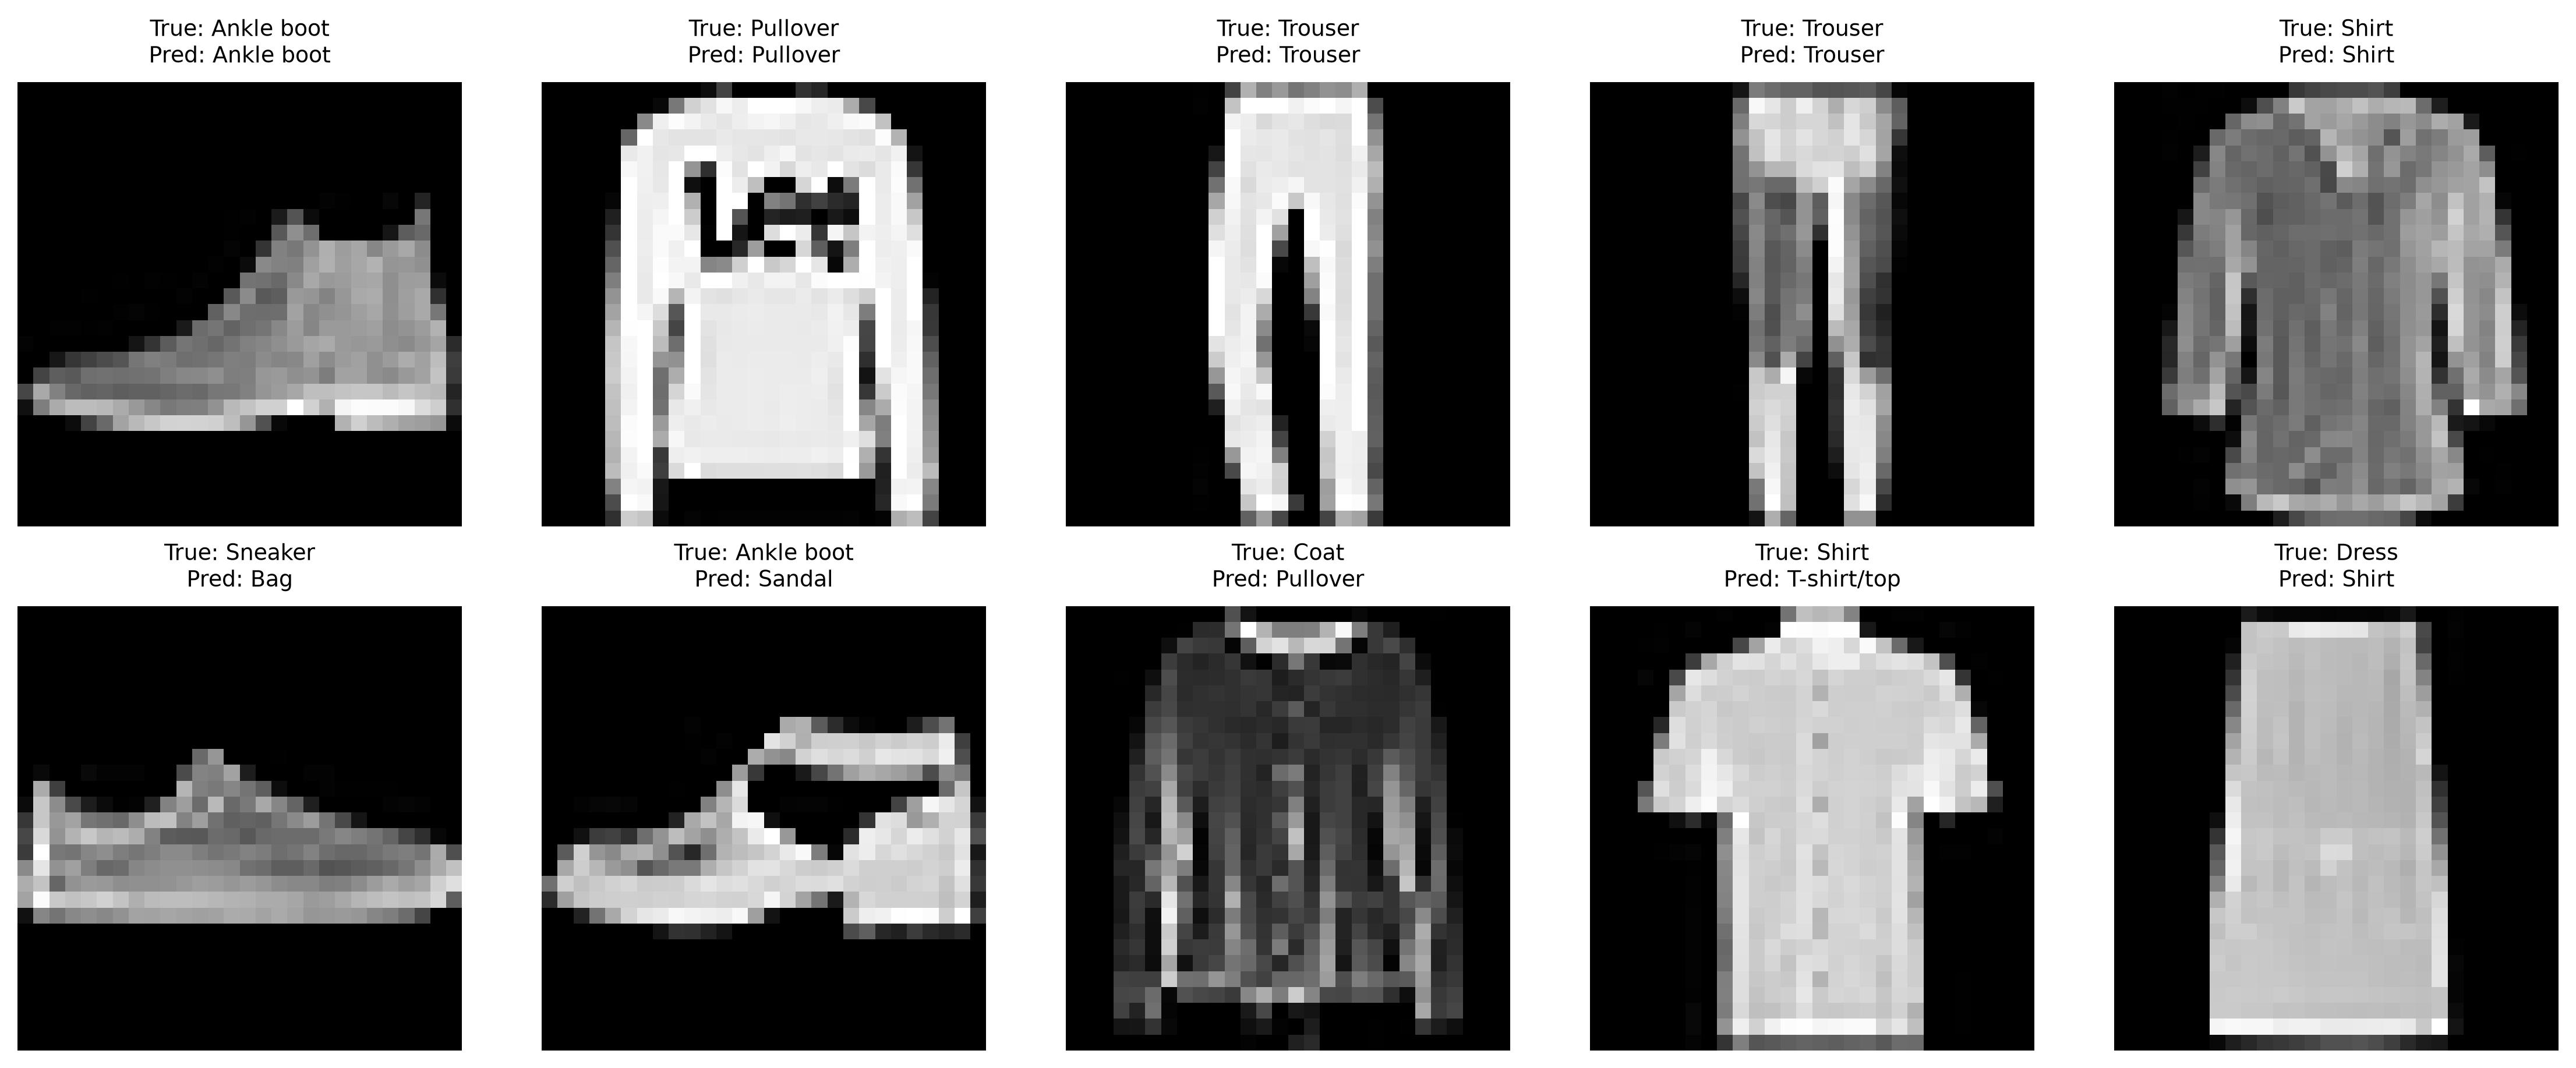
\includegraphics[width=\linewidth]{images/final_cnn_prediction_examples.png}

\captionof{figure}{Original CNN prediction-example image from branch \texttt{a1}. Five correct predictions appear above five failures; ground-truth and predicted labels are preserved.}

\label{fig:cnnexamples}

\end{minipage}\par\medskip



\par\medskip\noindent\begin{minipage}{\linewidth}
\centering
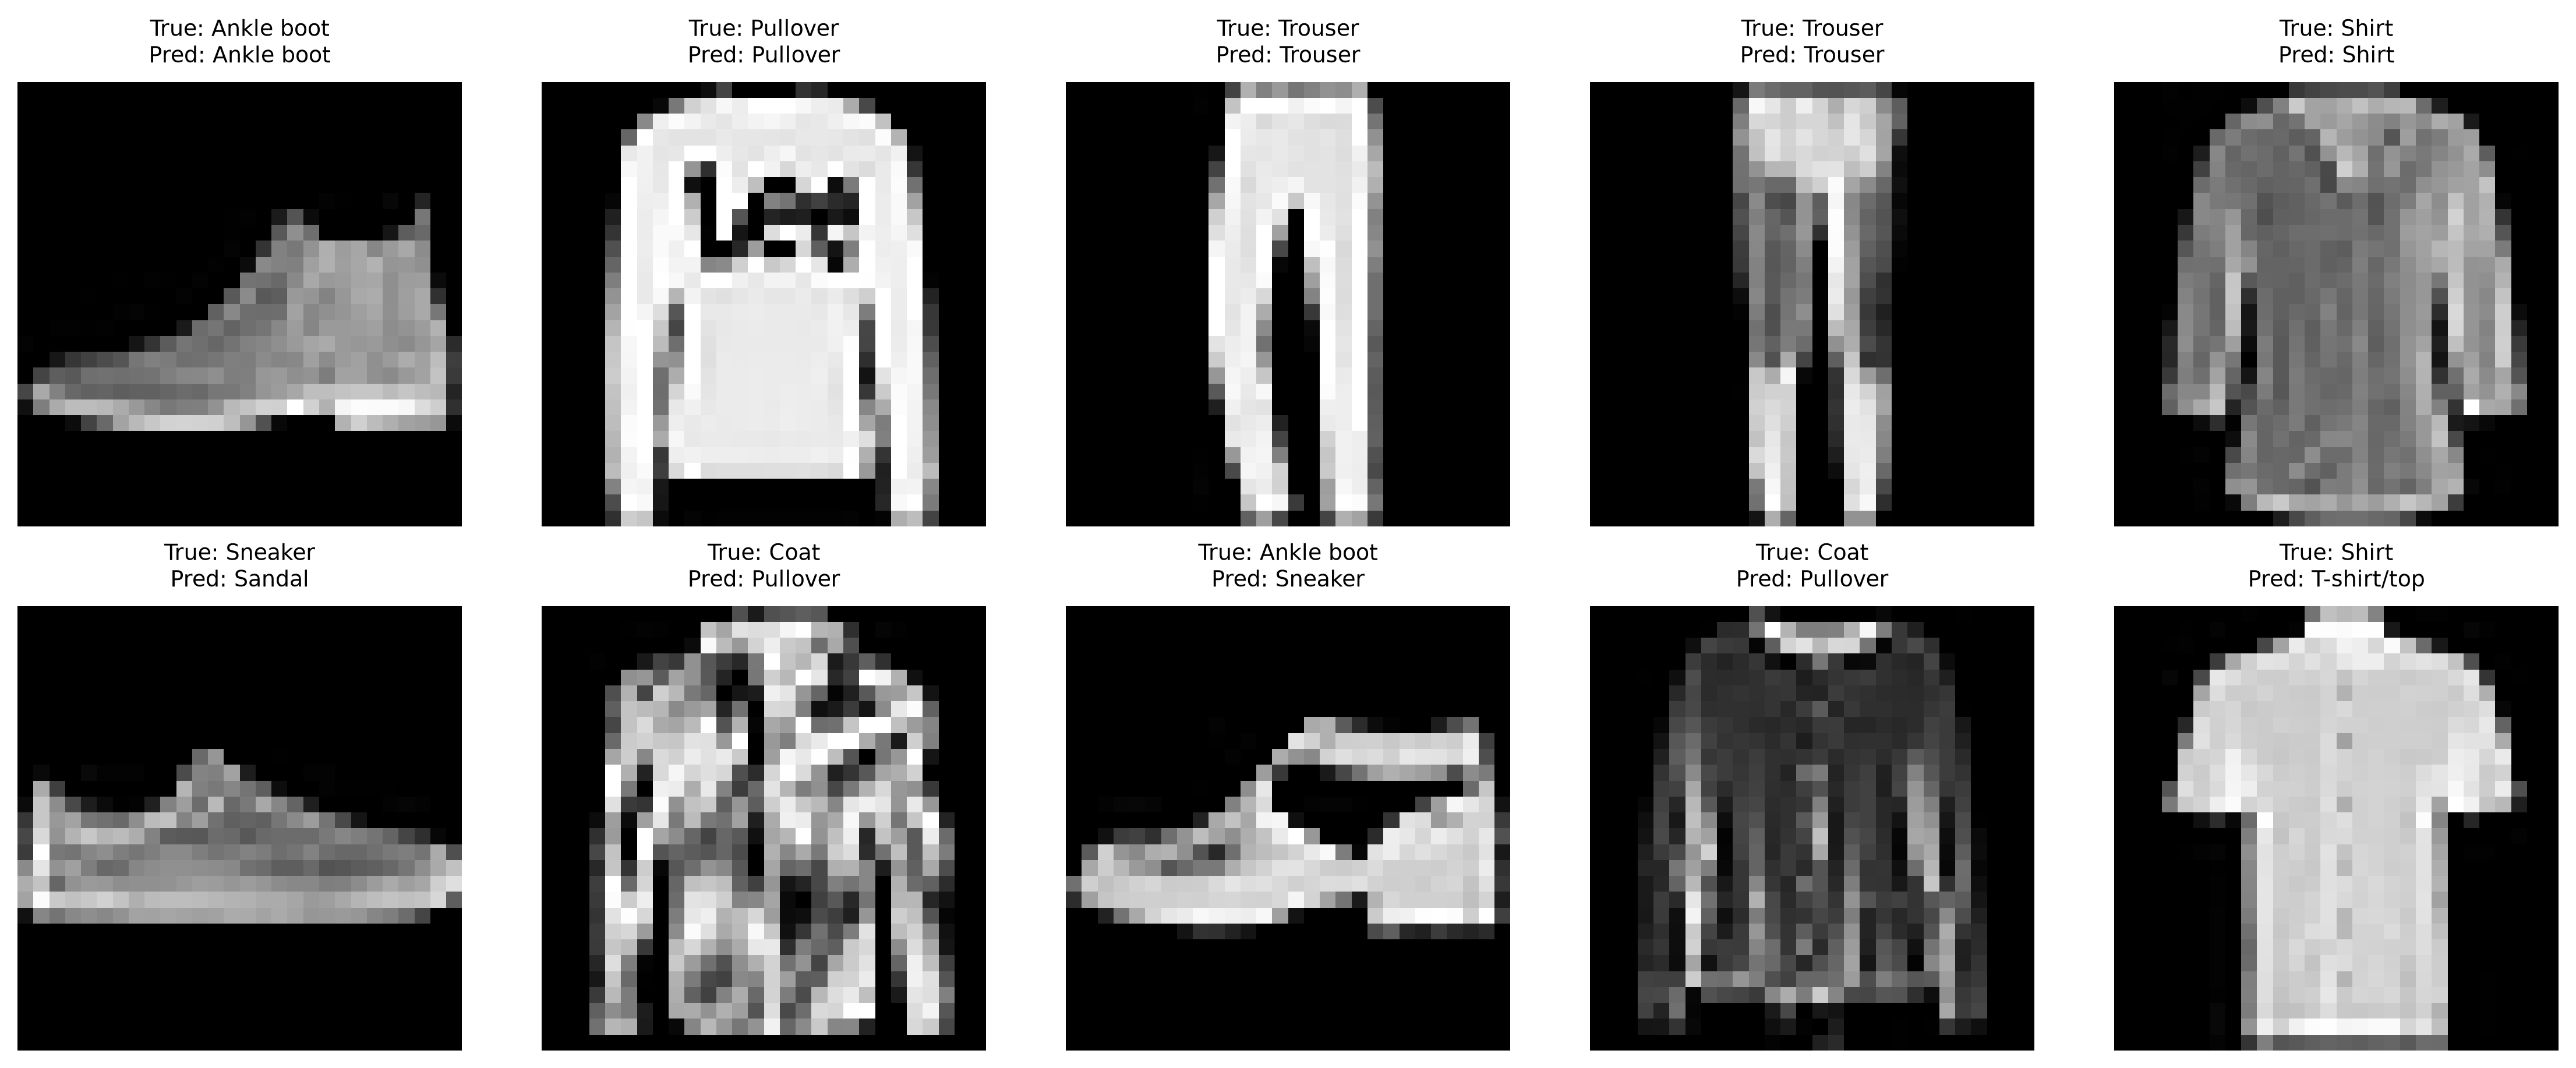
\includegraphics[width=\linewidth,height=.24\textheight,keepaspectratio]{images/final_linear_prediction_examples.png}
\captionof{figure}{Linear: original prediction examples from the selected branch run. Five correct predictions appear above five failures, with ground-truth and prediction labels.}
\label{fig:examples-linear}
\end{minipage}\par\medskip

\par\medskip\noindent\begin{minipage}{\linewidth}
\centering
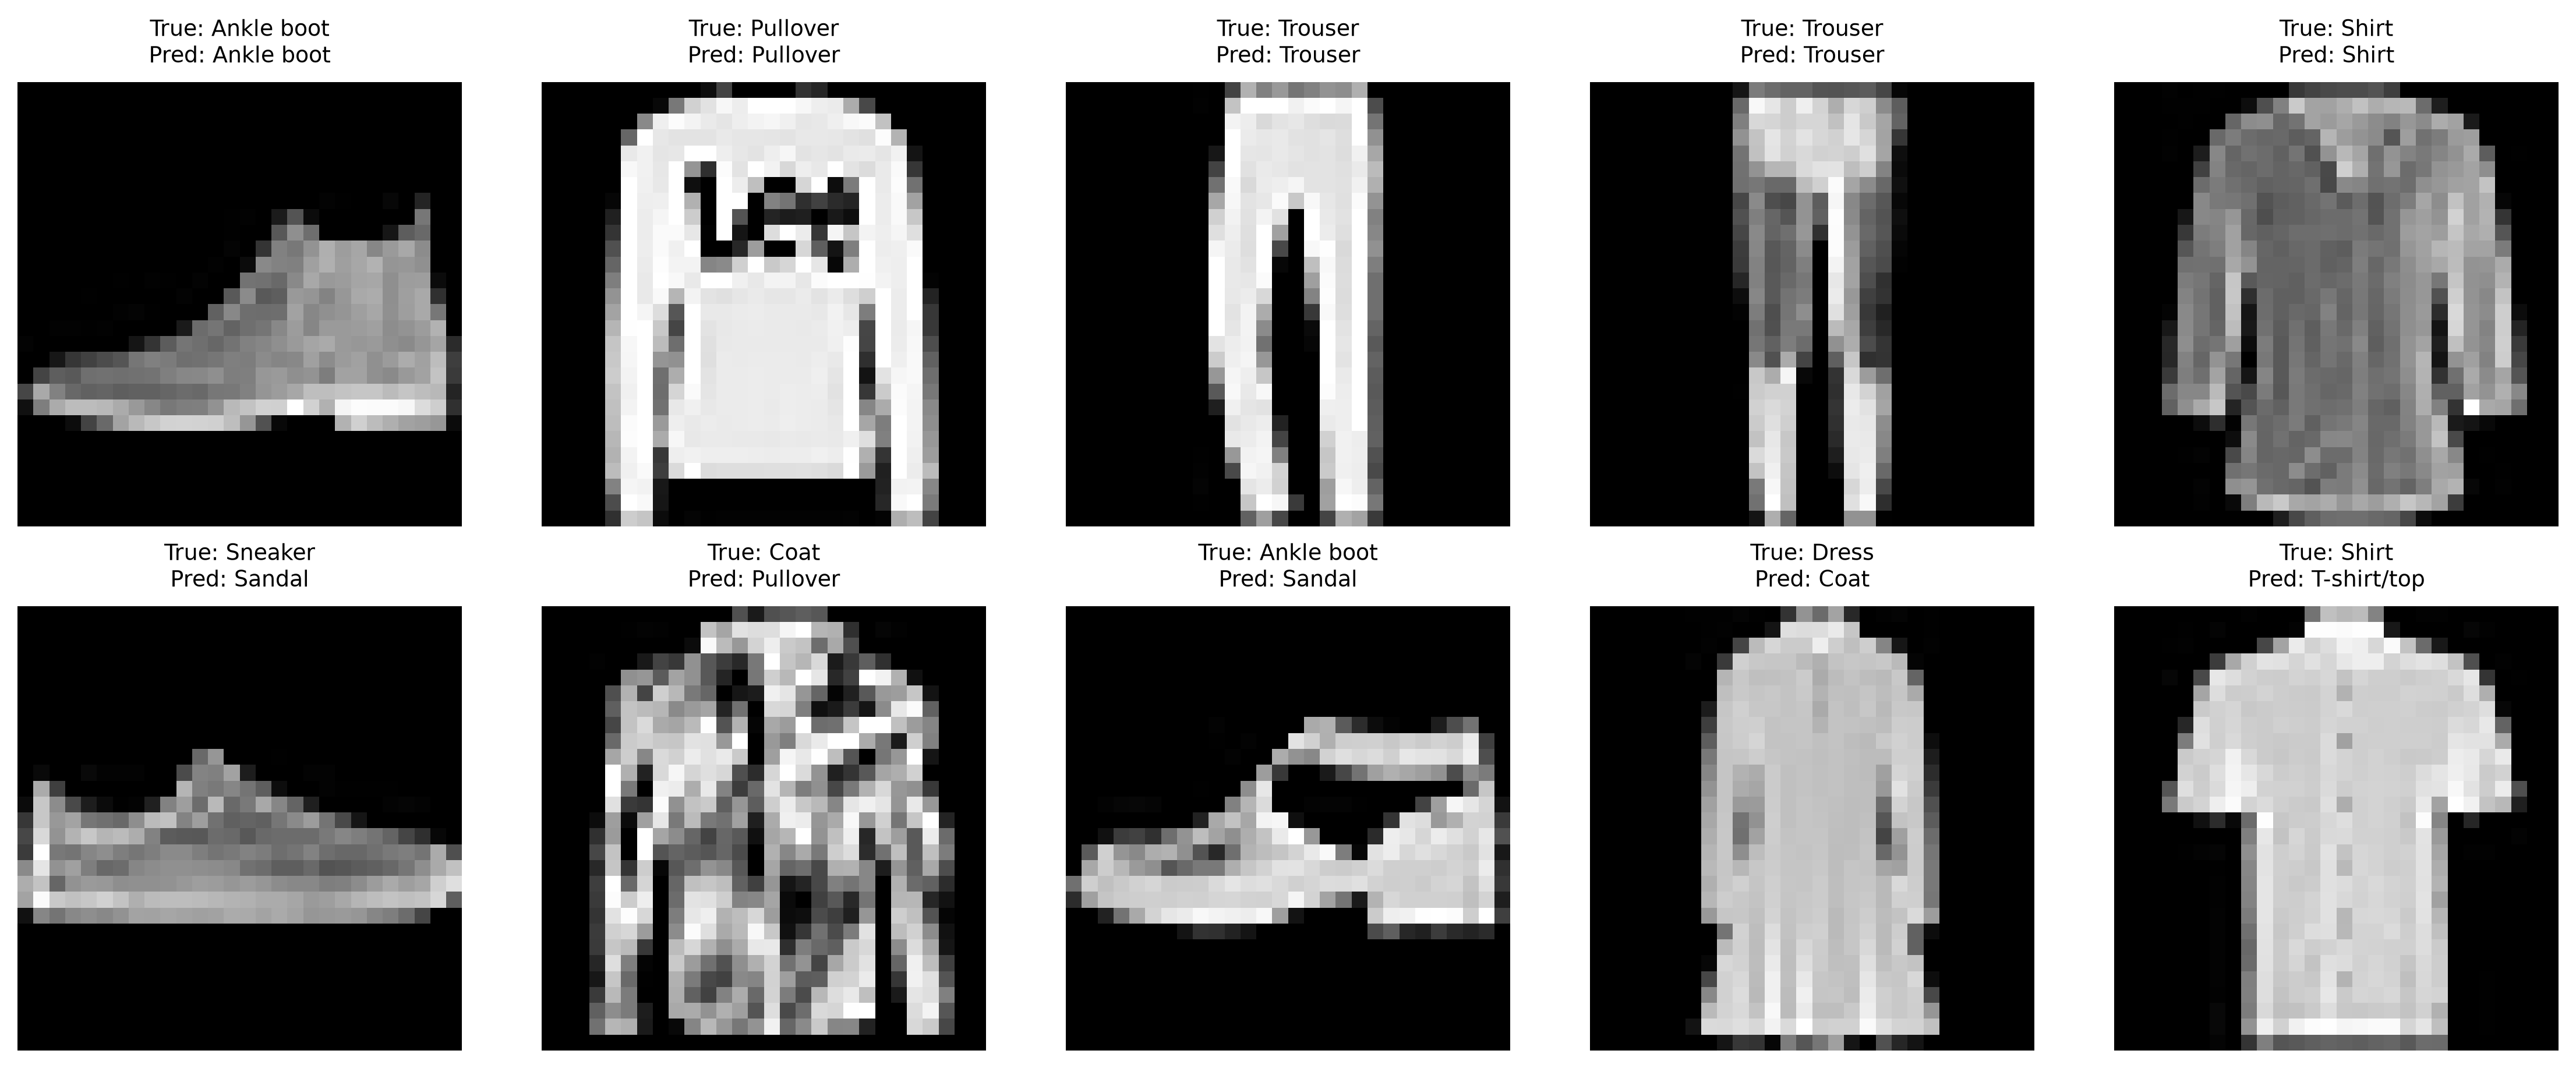
\includegraphics[width=\linewidth,height=.24\textheight,keepaspectratio]{images/final_mlp_prediction_examples.png}
\captionof{figure}{MLP: original prediction examples from the selected branch run. Five correct predictions appear above five failures, with ground-truth and prediction labels.}
\label{fig:examples-mlp}
\end{minipage}\par\medskip

\par\medskip\noindent\begin{minipage}{\linewidth}
\centering
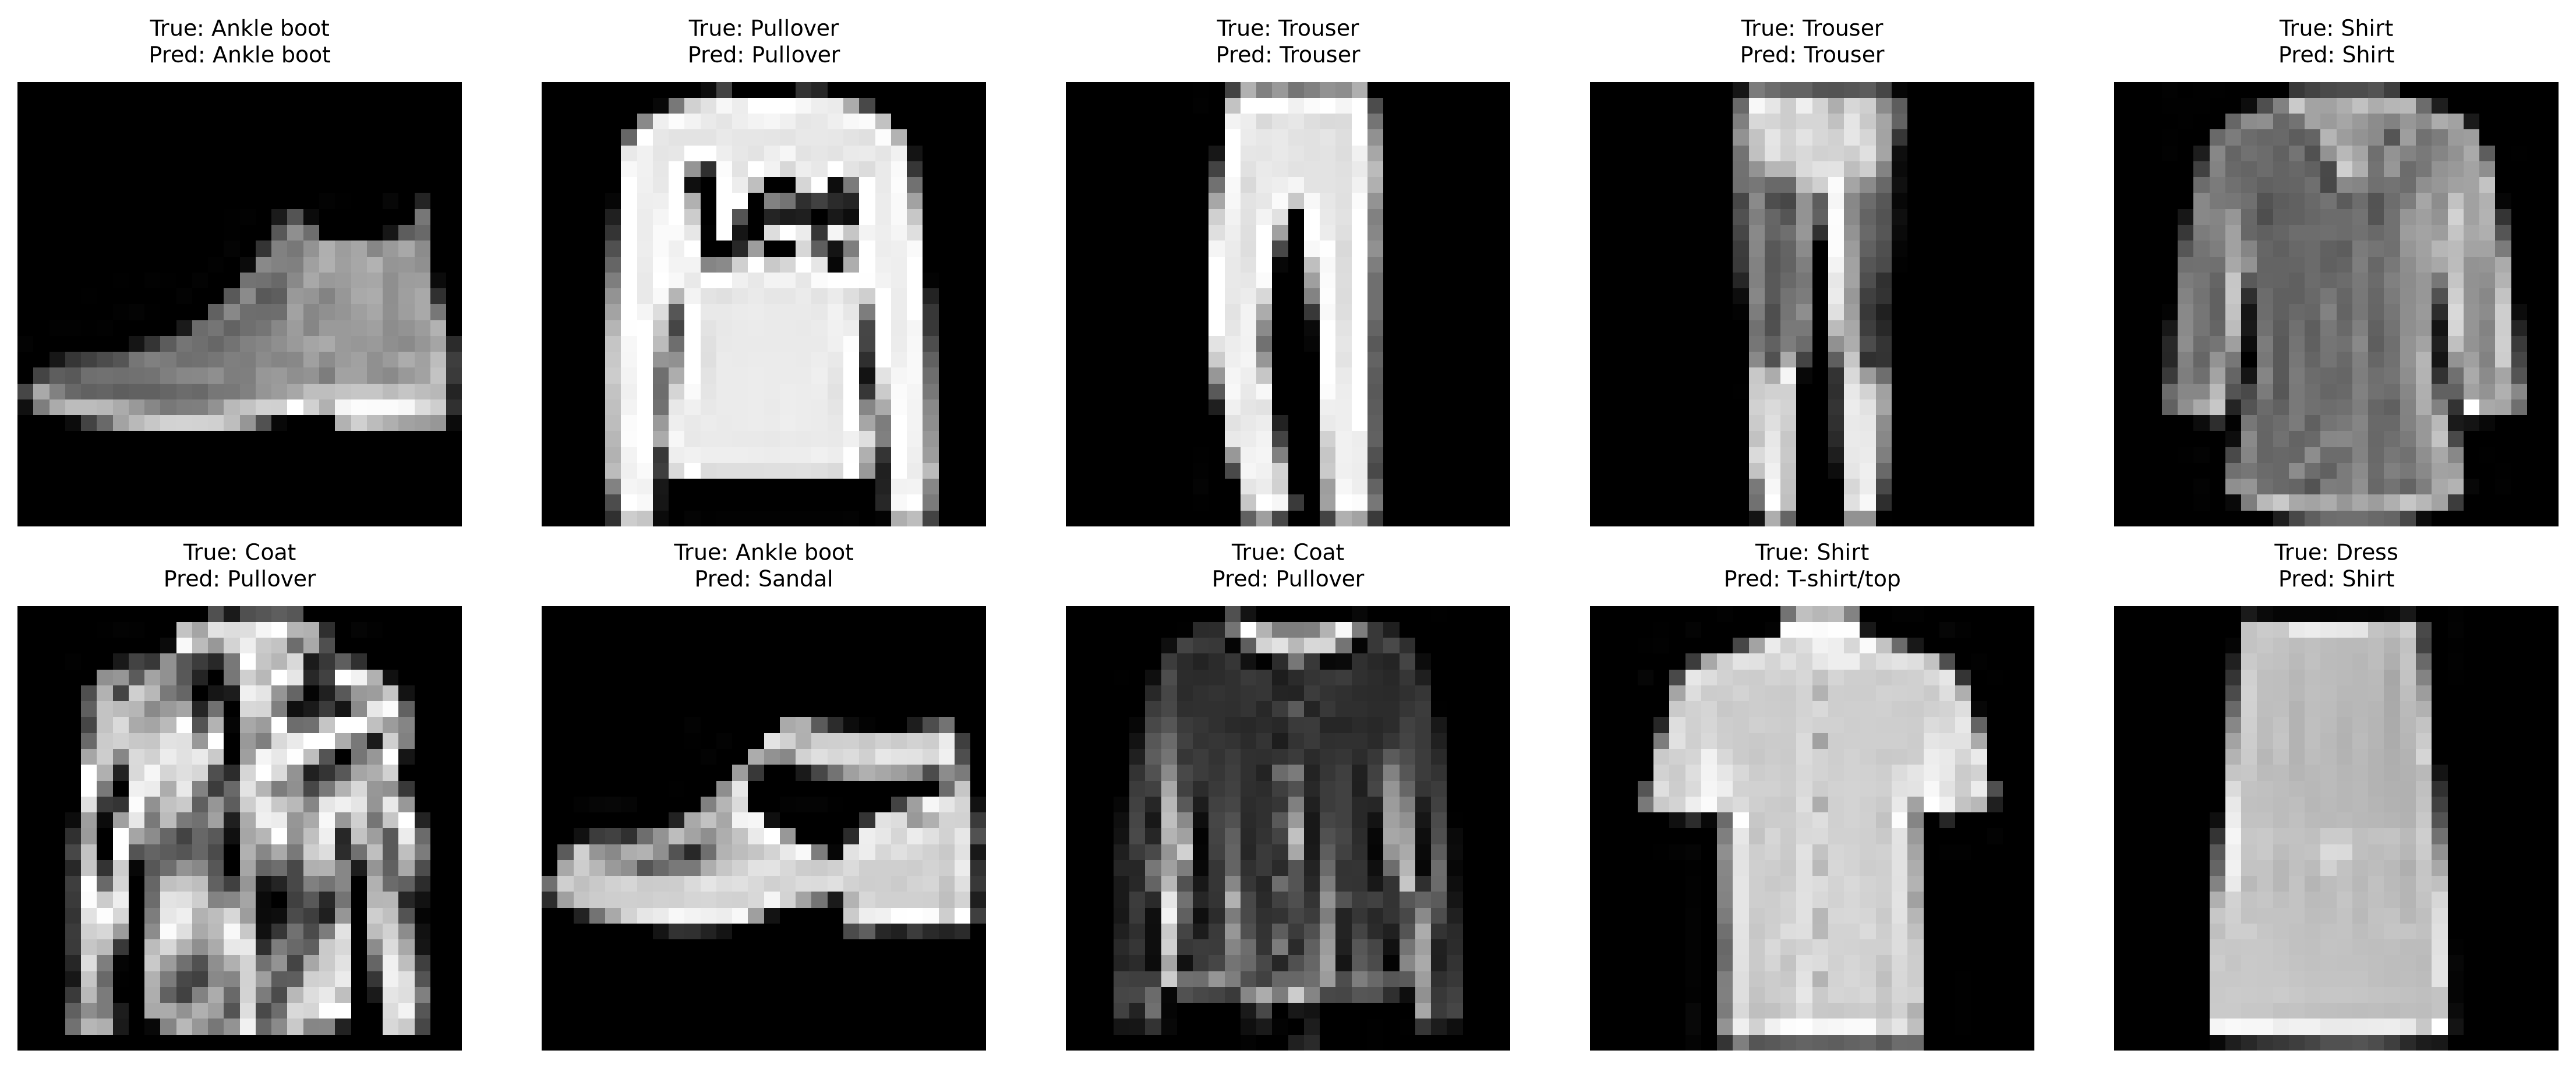
\includegraphics[width=\linewidth,height=.24\textheight,keepaspectratio]{images/final_lstm_prediction_examples.png}
\captionof{figure}{LSTM: original prediction examples from the selected branch run. Five correct predictions appear above five failures, with ground-truth and prediction labels.}
\label{fig:examples-lstm}
\end{minipage}\par\medskip

\par\medskip\noindent\begin{minipage}{\linewidth}
\centering
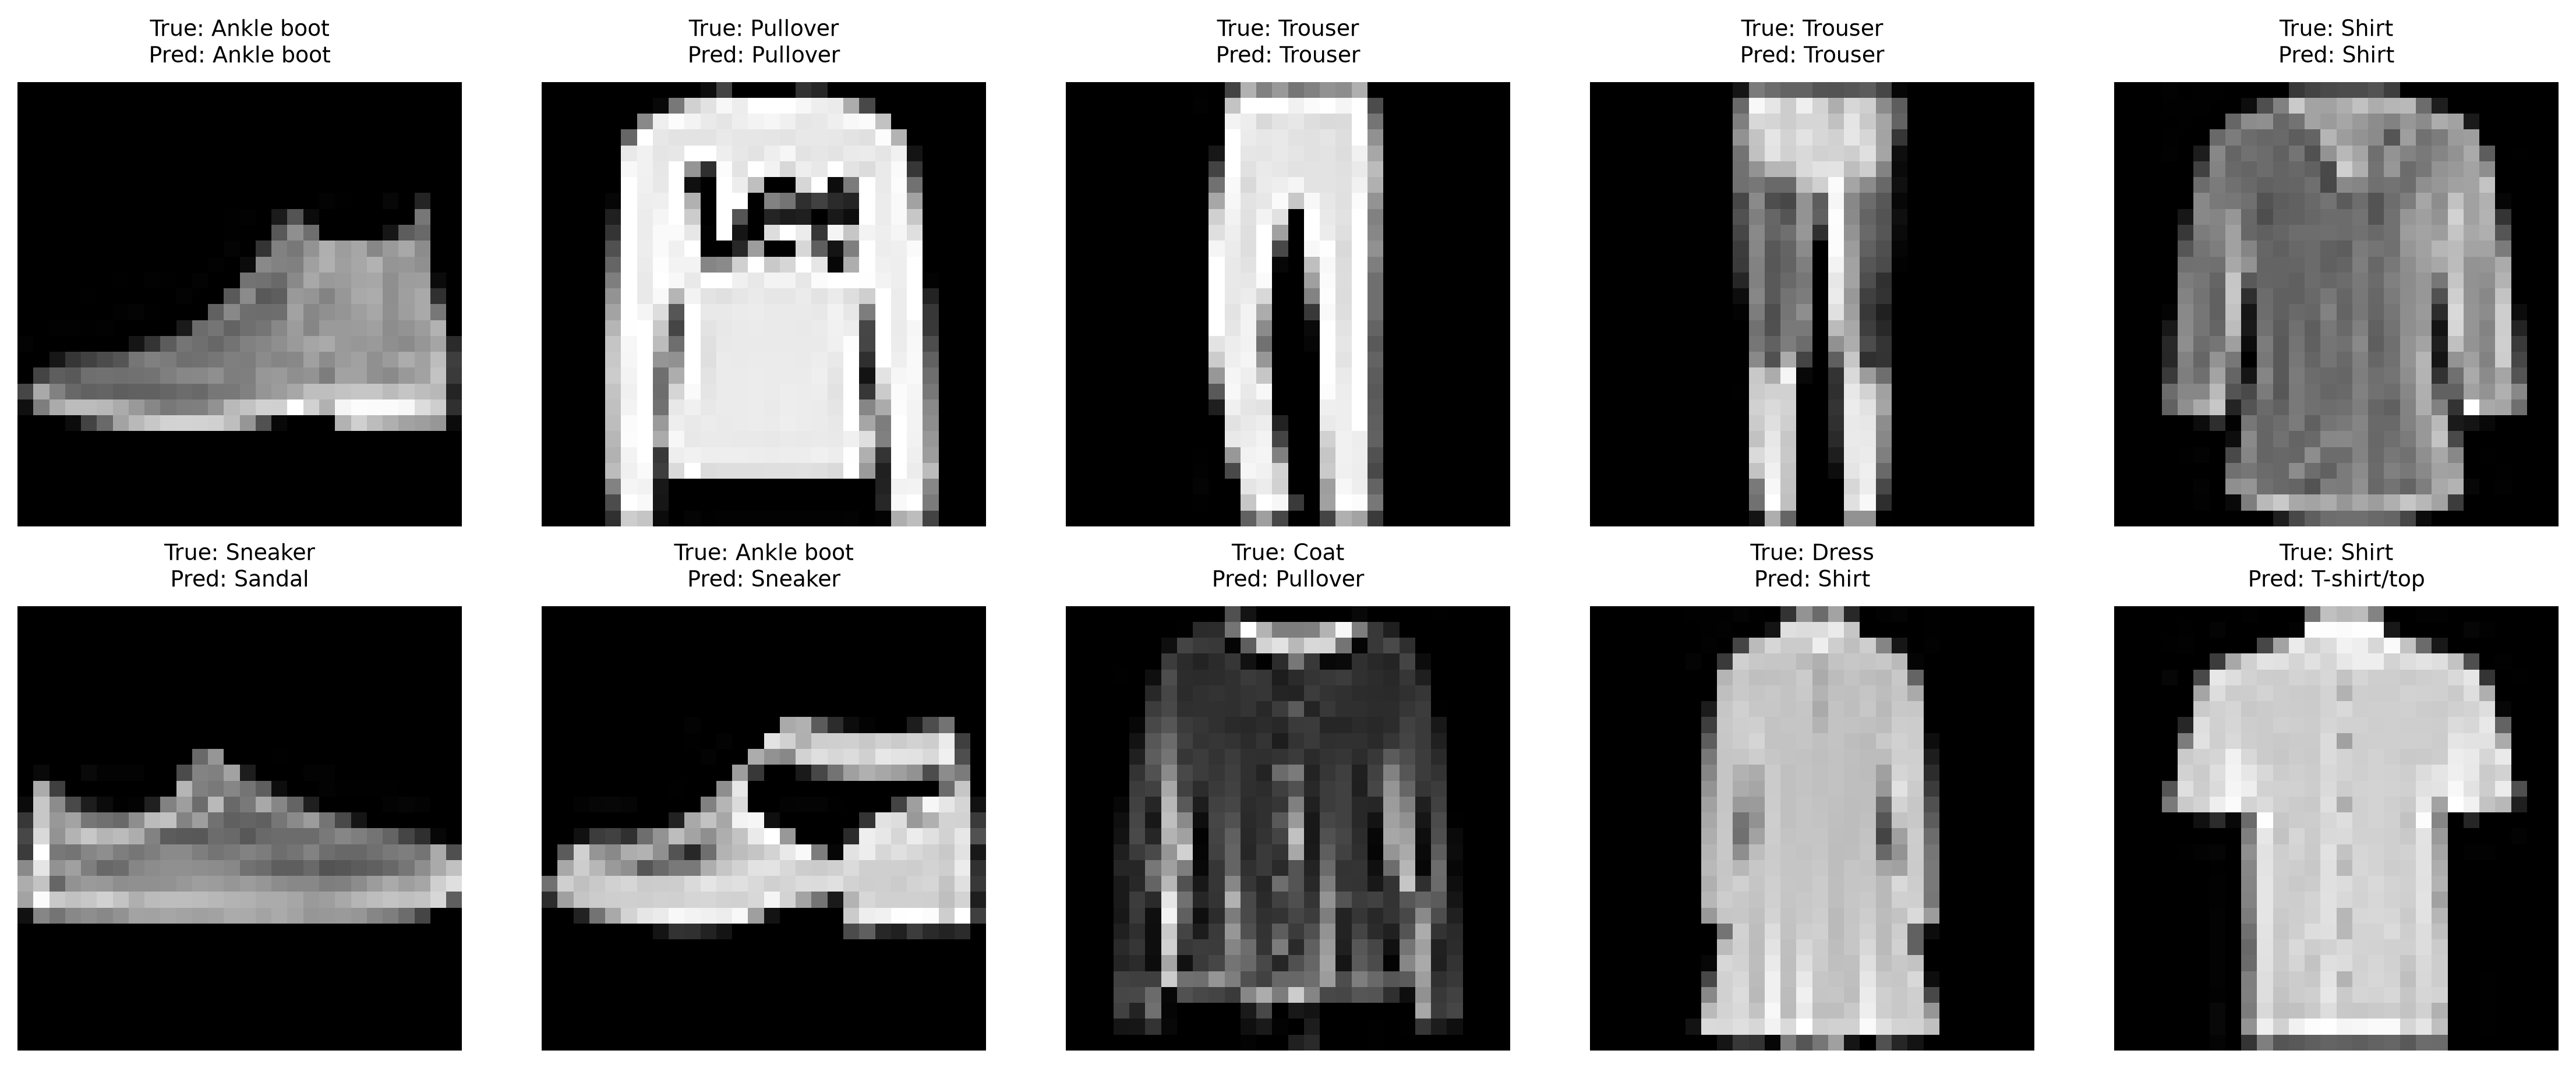
\includegraphics[width=\linewidth,height=.24\textheight,keepaspectratio]{images/final_transformer_prediction_examples.png}
\captionof{figure}{Transformer: original prediction examples from the selected branch run. Five correct predictions appear above five failures, with ground-truth and prediction labels.}
\label{fig:examples-transformer}
\end{minipage}\par\medskip

\subsection{Representation and Inductive Bias}

\subsubsection{Evidence for the Research Hypotheses}

\begin{itemize}
\setlength{\itemsep}{3pt}
\setlength{\parskip}{0pt}
\item \textbf{Nonlinear capacity.} The MLP exceeds Linear by 4.77 percentage points and 0.0482 Macro-F1, consistent with useful nonlinear pixel interactions.
\item \textbf{Spatial structure.} CNN then improves over MLP while using slightly fewer parameters, consistent with a beneficial image-specific bias from local receptive fields and weight sharing.
\item \textbf{Scope of evidence.} The comparison supports those hypotheses for these configurations; it does not isolate a causal contribution of each design choice because capacity, depth and operations also change.

\item \textbf{Row representation.} Row-wise LSTM processing improves over the flattened MLP slightly in aggregate, but its serial recurrence is expensive on the measured CPU. It does not preserve a two-dimensional neighborhood in the same explicit way as convolution.
\item \textbf{Patch representation.} Transformer can exchange information globally among 16 patches, but the learned representation and common 20-epoch budget yield a weaker result here.
\item \textbf{Observed ranking.} The evidence does not support the claim that a more modern or more parameter-rich architecture must outperform a small CNN on this benchmark.
\end{itemize}


\subsubsection{Practical Trade-Off}

\begin{itemize}
\setlength{\itemsep}{3pt}
\setlength{\parskip}{0pt}
\item \textbf{Quality priority.} CNN is the preferred quality-focused model among these runs.
\item \textbf{Latency priority.} If CPU forward latency is the principal constraint, MLP offers 89.08\% Accuracy at roughly one quarter of CNN's median time; Linear offers a still cheaper but less accurate reference.
\item \textbf{Sequence-model trade-off.} LSTM's small gain over MLP comes with a large cost, while Transformer is dominated by CNN in quality, parameters, training time and median inference time. This conclusion is specific to the recorded CPU protocol and saved configurations.
\end{itemize}


\subsection{Error Analysis}

\subsubsection{Frequent CNN Confusions}

\begin{table}[!htbp]\centering\small

\caption{Largest directed CNN confusions. Class rate uses 1,000 true-class examples; error share uses all 831 CNN mistakes.}

\label{tab:cnnerrors}

\begin{tabular}{@{}lrrr@{}}\toprule

True $\to$ predicted & Count & Class rate & Error share\\\midrule

Shirt $\to$ T-shirt/top & 100 & 10.0\% & 12.03\% \\

T-shirt/top $\to$ Shirt & 88 & 8.8\% & 10.59\% \\

Shirt $\to$ Pullover & 80 & 8.0\% & 9.63\% \\

Shirt $\to$ Coat & 72 & 7.2\% & 8.66\% \\

Coat $\to$ Pullover & 62 & 6.2\% & 7.46\% \\

\bottomrule\end{tabular}\end{table}



\begin{itemize}
\setlength{\itemsep}{3pt}
\setlength{\parskip}{0pt}
\item \textbf{Frequent directions.} The five listed directions account for 402 mistakes (48.4\% of all CNN errors).
\item \textbf{Upper-body confusion.} Four upper-body classes---T-shirt/top, Pullover, Coat and Shirt---contain 547 internal off-diagonal confusions, or 65.8\% of all errors.
\item \textbf{Shirt errors.} The 288 Shirt false negatives alone contribute 34.7\% of errors; 252 of them go to the other three upper-body categories. This concentration is more informative than the overall 8.31\% error rate.

\item \textbf{Baseline comparison.} Linear's largest directions include Shirt-to-T-shirt/top (153) and Pullover-to-Coat (150).
\item \textbf{Asymmetric errors.} CNN reduces these to 100 and 35, while some directions remain asymmetric: 100 shirts become T-shirt/top, versus 88 T-shirt/top images becoming Shirt. Predicted-class frequency and decision boundaries matter alongside raw visual resemblance.
\end{itemize}


\subsubsection{Interpretation of the Observed Errors}

\begin{itemize}
\setlength{\itemsep}{3pt}
\setlength{\parskip}{0pt}
\item \textbf{Plausible sources.} Shared silhouettes, low resolution and missing color/texture plausibly contribute to upper-body confusion.
\item \textbf{Evidence limits.} These are interpretations consistent with the class-level pattern, not measured causal effects or evidence that labels are wrong.
\item \textbf{Other failure types.} Garment boundaries, sleeve shape and fine texture could be less distinctive after downsampling and pooling. The illustrative prediction panels also contain rare errors outside this dominant group, so error analysis should not focus exclusively on one pair.
\end{itemize}


\subsection{Conclusion}

The completed shared pipeline supports five architecture families and traceable test evaluation. CNN gives the best observed quality (91.69\% Accuracy, 0.9163 Macro-F1), with 47.0\% fewer errors than Linear and 23.9\% fewer than MLP. Its local image structure is effective for this small grayscale benchmark, although its measured forward cost exceeds that of the dense baselines. MLP supplies a useful accuracy--latency compromise. Sequence models are functional, but their greater flexibility does not yield the best quality/cost trade-off here.



The comparison uses one seed, architecture-dependent parameter counts, a common 20-epoch budget and a forward-only CPU benchmark with 20 timed repeats. Split checks address index leakage rather than visual duplicates. Fashion-MNIST does not establish robustness to unrestricted photographs or unseen classes.

